% Created by tikzDevice version 0.12.4 on 2023-03-21 21:56:14
% !TEX encoding = UTF-8 Unicode
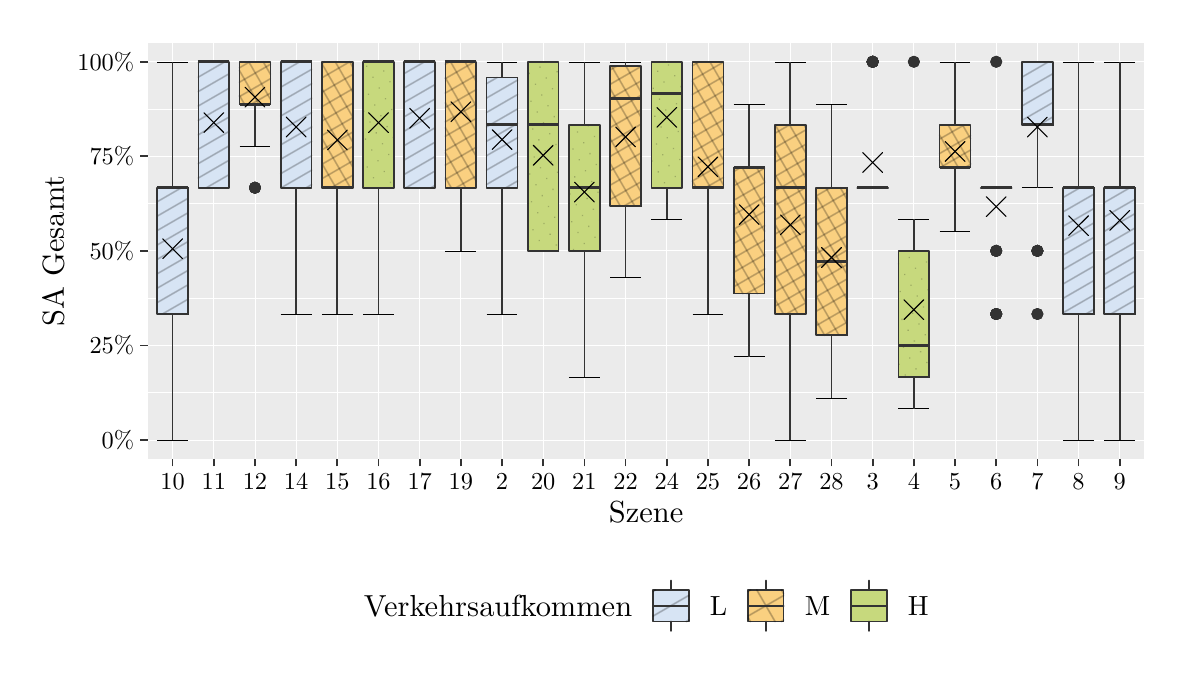
\begin{tikzpicture}[x=1pt,y=1pt]
\definecolor{fillColor}{RGB}{255,255,255}
\path[use as bounding box,fill=fillColor,fill opacity=0.00] (0,0) rectangle (409.05,231.26);
\begin{scope}
\path[clip] (  0.00,  0.00) rectangle (409.05,231.26);
\definecolor{drawColor}{RGB}{255,255,255}
\definecolor{fillColor}{RGB}{255,255,255}

\path[draw=drawColor,line width= 0.6pt,line join=round,line cap=round,fill=fillColor] (  0.00, -0.00) rectangle (409.05,231.26);
\end{scope}
\begin{scope}
\path[clip] ( 43.44, 75.45) rectangle (403.55,225.76);
\definecolor{fillColor}{gray}{0.92}

\path[fill=fillColor] ( 43.44, 75.45) rectangle (403.55,225.76);
\definecolor{drawColor}{RGB}{255,255,255}

\path[draw=drawColor,line width= 0.3pt,line join=round] ( 43.44, 99.36) --
	(403.55, 99.36);

\path[draw=drawColor,line width= 0.3pt,line join=round] ( 43.44,133.52) --
	(403.55,133.52);

\path[draw=drawColor,line width= 0.3pt,line join=round] ( 43.44,167.69) --
	(403.55,167.69);

\path[draw=drawColor,line width= 0.3pt,line join=round] ( 43.44,201.85) --
	(403.55,201.85);

\path[draw=drawColor,line width= 0.3pt,line join=round] ( 43.44, 82.28) --
	(403.55, 82.28);

\path[draw=drawColor,line width= 0.3pt,line join=round] ( 43.44,116.44) --
	(403.55,116.44);

\path[draw=drawColor,line width= 0.3pt,line join=round] ( 43.44,150.61) --
	(403.55,150.61);

\path[draw=drawColor,line width= 0.3pt,line join=round] ( 43.44,184.77) --
	(403.55,184.77);

\path[draw=drawColor,line width= 0.3pt,line join=round] ( 43.44,218.93) --
	(403.55,218.93);

\path[draw=drawColor,line width= 0.3pt,line join=round] ( 52.37, 75.45) --
	( 52.37,225.76);

\path[draw=drawColor,line width= 0.3pt,line join=round] ( 67.25, 75.45) --
	( 67.25,225.76);

\path[draw=drawColor,line width= 0.3pt,line join=round] ( 82.13, 75.45) --
	( 82.13,225.76);

\path[draw=drawColor,line width= 0.3pt,line join=round] ( 97.01, 75.45) --
	( 97.01,225.76);

\path[draw=drawColor,line width= 0.3pt,line join=round] (111.89, 75.45) --
	(111.89,225.76);

\path[draw=drawColor,line width= 0.3pt,line join=round] (126.77, 75.45) --
	(126.77,225.76);

\path[draw=drawColor,line width= 0.3pt,line join=round] (141.65, 75.45) --
	(141.65,225.76);

\path[draw=drawColor,line width= 0.3pt,line join=round] (156.53, 75.45) --
	(156.53,225.76);

\path[draw=drawColor,line width= 0.3pt,line join=round] (171.41, 75.45) --
	(171.41,225.76);

\path[draw=drawColor,line width= 0.3pt,line join=round] (186.29, 75.45) --
	(186.29,225.76);

\path[draw=drawColor,line width= 0.3pt,line join=round] (201.17, 75.45) --
	(201.17,225.76);

\path[draw=drawColor,line width= 0.3pt,line join=round] (216.06, 75.45) --
	(216.06,225.76);

\path[draw=drawColor,line width= 0.3pt,line join=round] (230.94, 75.45) --
	(230.94,225.76);

\path[draw=drawColor,line width= 0.3pt,line join=round] (245.82, 75.45) --
	(245.82,225.76);

\path[draw=drawColor,line width= 0.3pt,line join=round] (260.70, 75.45) --
	(260.70,225.76);

\path[draw=drawColor,line width= 0.3pt,line join=round] (275.58, 75.45) --
	(275.58,225.76);

\path[draw=drawColor,line width= 0.3pt,line join=round] (290.46, 75.45) --
	(290.46,225.76);

\path[draw=drawColor,line width= 0.3pt,line join=round] (305.34, 75.45) --
	(305.34,225.76);

\path[draw=drawColor,line width= 0.3pt,line join=round] (320.22, 75.45) --
	(320.22,225.76);

\path[draw=drawColor,line width= 0.3pt,line join=round] (335.10, 75.45) --
	(335.10,225.76);

\path[draw=drawColor,line width= 0.3pt,line join=round] (349.98, 75.45) --
	(349.98,225.76);

\path[draw=drawColor,line width= 0.3pt,line join=round] (364.86, 75.45) --
	(364.86,225.76);

\path[draw=drawColor,line width= 0.3pt,line join=round] (379.74, 75.45) --
	(379.74,225.76);

\path[draw=drawColor,line width= 0.3pt,line join=round] (394.62, 75.45) --
	(394.62,225.76);
\definecolor{drawColor}{RGB}{0,0,0}

\path[draw=drawColor,line width= 0.2pt,line join=round] ( 46.79,218.93) --
	( 57.95,218.93);

\path[draw=drawColor,line width= 0.2pt,line join=round] ( 52.37,218.93) --
	( 52.37, 82.28);

\path[draw=drawColor,line width= 0.2pt,line join=round] ( 46.79, 82.28) --
	( 57.95, 82.28);

\path[draw=drawColor,line width= 0.2pt,line join=round] ( 61.67,218.93) --
	( 72.83,218.93);

\path[draw=drawColor,line width= 0.2pt,line join=round] ( 67.25,218.93) --
	( 67.25,173.43);

\path[draw=drawColor,line width= 0.2pt,line join=round] ( 61.67,173.43) --
	( 72.83,173.43);

\path[draw=drawColor,line width= 0.2pt,line join=round] ( 76.55,218.93) --
	( 87.71,218.93);

\path[draw=drawColor,line width= 0.2pt,line join=round] ( 82.13,218.93) --
	( 82.13,188.46);

\path[draw=drawColor,line width= 0.2pt,line join=round] ( 76.55,188.46) --
	( 87.71,188.46);

\path[draw=drawColor,line width= 0.2pt,line join=round] ( 91.43,218.93) --
	(102.59,218.93);

\path[draw=drawColor,line width= 0.2pt,line join=round] ( 97.01,218.93) --
	( 97.01,127.79);

\path[draw=drawColor,line width= 0.2pt,line join=round] ( 91.43,127.79) --
	(102.59,127.79);

\path[draw=drawColor,line width= 0.2pt,line join=round] (106.31,218.93) --
	(117.47,218.93);

\path[draw=drawColor,line width= 0.2pt,line join=round] (111.89,218.93) --
	(111.89,127.79);

\path[draw=drawColor,line width= 0.2pt,line join=round] (106.31,127.79) --
	(117.47,127.79);

\path[draw=drawColor,line width= 0.2pt,line join=round] (121.19,218.93) --
	(132.35,218.93);

\path[draw=drawColor,line width= 0.2pt,line join=round] (126.77,218.93) --
	(126.77,127.79);

\path[draw=drawColor,line width= 0.2pt,line join=round] (121.19,127.79) --
	(132.35,127.79);

\path[draw=drawColor,line width= 0.2pt,line join=round] (136.07,218.93) --
	(147.23,218.93);

\path[draw=drawColor,line width= 0.2pt,line join=round] (141.65,218.93) --
	(141.65,173.43);

\path[draw=drawColor,line width= 0.2pt,line join=round] (136.07,173.43) --
	(147.23,173.43);

\path[draw=drawColor,line width= 0.2pt,line join=round] (150.95,218.93) --
	(162.11,218.93);

\path[draw=drawColor,line width= 0.2pt,line join=round] (156.53,218.93) --
	(156.53,150.61);

\path[draw=drawColor,line width= 0.2pt,line join=round] (150.95,150.61) --
	(162.11,150.61);

\path[draw=drawColor,line width= 0.2pt,line join=round] (165.83,218.93) --
	(176.99,218.93);

\path[draw=drawColor,line width= 0.2pt,line join=round] (171.41,218.93) --
	(171.41,127.79);

\path[draw=drawColor,line width= 0.2pt,line join=round] (165.83,127.79) --
	(176.99,127.79);

\path[draw=drawColor,line width= 0.2pt,line join=round] (180.71,218.93) --
	(191.87,218.93);

\path[draw=drawColor,line width= 0.2pt,line join=round] (186.29,218.93) --
	(186.29,150.61);

\path[draw=drawColor,line width= 0.2pt,line join=round] (180.71,150.61) --
	(191.87,150.61);

\path[draw=drawColor,line width= 0.2pt,line join=round] (195.59,218.93) --
	(206.76,218.93);

\path[draw=drawColor,line width= 0.2pt,line join=round] (201.17,218.93) --
	(201.17,105.10);

\path[draw=drawColor,line width= 0.2pt,line join=round] (195.59,105.10) --
	(206.76,105.10);

\path[draw=drawColor,line width= 0.2pt,line join=round] (210.48,218.93) --
	(221.64,218.93);

\path[draw=drawColor,line width= 0.2pt,line join=round] (216.06,218.93) --
	(216.06,141.04);

\path[draw=drawColor,line width= 0.2pt,line join=round] (210.48,141.04) --
	(221.64,141.04);

\path[draw=drawColor,line width= 0.2pt,line join=round] (225.36,218.93) --
	(236.52,218.93);

\path[draw=drawColor,line width= 0.2pt,line join=round] (230.94,218.93) --
	(230.94,161.95);

\path[draw=drawColor,line width= 0.2pt,line join=round] (225.36,161.95) --
	(236.52,161.95);

\path[draw=drawColor,line width= 0.2pt,line join=round] (240.24,218.93) --
	(251.40,218.93);

\path[draw=drawColor,line width= 0.2pt,line join=round] (245.82,218.93) --
	(245.82,127.79);

\path[draw=drawColor,line width= 0.2pt,line join=round] (240.24,127.79) --
	(251.40,127.79);

\path[draw=drawColor,line width= 0.2pt,line join=round] (255.12,203.49) --
	(266.28,203.49);

\path[draw=drawColor,line width= 0.2pt,line join=round] (260.70,203.49) --
	(260.70,112.34);

\path[draw=drawColor,line width= 0.2pt,line join=round] (255.12,112.34) --
	(266.28,112.34);

\path[draw=drawColor,line width= 0.2pt,line join=round] (270.00,218.93) --
	(281.16,218.93);

\path[draw=drawColor,line width= 0.2pt,line join=round] (275.58,218.93) --
	(275.58, 82.28);

\path[draw=drawColor,line width= 0.2pt,line join=round] (270.00, 82.28) --
	(281.16, 82.28);

\path[draw=drawColor,line width= 0.2pt,line join=round] (284.88,203.49) --
	(296.04,203.49);

\path[draw=drawColor,line width= 0.2pt,line join=round] (290.46,203.49) --
	(290.46, 97.31);

\path[draw=drawColor,line width= 0.2pt,line join=round] (284.88, 97.31) --
	(296.04, 97.31);

\path[draw=drawColor,line width= 0.2pt,line join=round] (299.76,173.43) --
	(310.92,173.43);

\path[draw=drawColor,line width= 0.2pt,line join=round] (305.34,173.43) --
	(305.34,173.43);

\path[draw=drawColor,line width= 0.2pt,line join=round] (299.76,173.43) --
	(310.92,173.43);

\path[draw=drawColor,line width= 0.2pt,line join=round] (314.64,161.95) --
	(325.80,161.95);

\path[draw=drawColor,line width= 0.2pt,line join=round] (320.22,161.95) --
	(320.22, 93.62);

\path[draw=drawColor,line width= 0.2pt,line join=round] (314.64, 93.62) --
	(325.80, 93.62);

\path[draw=drawColor,line width= 0.2pt,line join=round] (329.52,218.93) --
	(340.68,218.93);

\path[draw=drawColor,line width= 0.2pt,line join=round] (335.10,218.93) --
	(335.10,157.85);

\path[draw=drawColor,line width= 0.2pt,line join=round] (329.52,157.85) --
	(340.68,157.85);

\path[draw=drawColor,line width= 0.2pt,line join=round] (344.40,173.43) --
	(355.56,173.43);

\path[draw=drawColor,line width= 0.2pt,line join=round] (349.98,173.43) --
	(349.98,173.43);

\path[draw=drawColor,line width= 0.2pt,line join=round] (344.40,173.43) --
	(355.56,173.43);

\path[draw=drawColor,line width= 0.2pt,line join=round] (359.28,218.93) --
	(370.44,218.93);

\path[draw=drawColor,line width= 0.2pt,line join=round] (364.86,218.93) --
	(364.86,173.43);

\path[draw=drawColor,line width= 0.2pt,line join=round] (359.28,173.43) --
	(370.44,173.43);

\path[draw=drawColor,line width= 0.2pt,line join=round] (374.16,218.93) --
	(385.32,218.93);

\path[draw=drawColor,line width= 0.2pt,line join=round] (379.74,218.93) --
	(379.74, 82.28);

\path[draw=drawColor,line width= 0.2pt,line join=round] (374.16, 82.28) --
	(385.32, 82.28);

\path[draw=drawColor,line width= 0.2pt,line join=round] (389.04,218.93) --
	(400.20,218.93);

\path[draw=drawColor,line width= 0.2pt,line join=round] (394.62,218.93) --
	(394.62, 82.28);

\path[draw=drawColor,line width= 0.2pt,line join=round] (389.04, 82.28) --
	(400.20, 82.28);
\definecolor{drawColor}{gray}{0.20}

\path[draw=drawColor,line width= 0.2pt,line join=round] ( 52.37,173.43) -- ( 52.37,218.93);

\path[draw=drawColor,line width= 0.2pt,line join=round] ( 52.37,127.79) -- ( 52.37, 82.28);
\definecolor{fillColor}{RGB}{215,228,244}

\path[draw=drawColor,line width= 0.2pt,fill=fillColor] ( 46.79,173.43) --
	( 46.79,127.79) --
	( 57.95,127.79) --
	( 57.95,173.43) --
	( 46.79,173.43) --
	cycle;

\path[draw=drawColor,line width= 0.5pt] ( 46.79,173.43) -- ( 57.95,173.43);

\path[draw=drawColor,line width= 0.2pt,line join=round] ( 67.25,218.93) -- ( 67.25,218.93);

\path[draw=drawColor,line width= 0.2pt,line join=round] ( 67.25,173.43) -- ( 67.25,173.43);

\path[draw=drawColor,line width= 0.2pt,fill=fillColor] ( 61.67,218.93) --
	( 61.67,173.43) --
	( 72.83,173.43) --
	( 72.83,218.93) --
	( 61.67,218.93) --
	cycle;

\path[draw=drawColor,line width= 0.5pt] ( 61.67,218.93) -- ( 72.83,218.93);
\definecolor{fillColor}{gray}{0.20}

\path[draw=drawColor,line width= 0.4pt,line join=round,line cap=round,fill=fillColor] ( 82.13,173.43) circle (  1.96);

\path[draw=drawColor,line width= 0.4pt,line join=round,line cap=round,fill=fillColor] ( 82.13,173.43) circle (  1.96);

\path[draw=drawColor,line width= 0.4pt,line join=round,line cap=round,fill=fillColor] ( 82.13,173.43) circle (  1.96);

\path[draw=drawColor,line width= 0.2pt,line join=round] ( 82.13,218.93) -- ( 82.13,218.93);

\path[draw=drawColor,line width= 0.2pt,line join=round] ( 82.13,203.49) -- ( 82.13,188.46);
\definecolor{fillColor}{RGB}{250,208,128}

\path[draw=drawColor,line width= 0.2pt,fill=fillColor] ( 76.55,218.93) --
	( 76.55,203.49) --
	( 87.71,203.49) --
	( 87.71,218.93) --
	( 76.55,218.93) --
	cycle;

\path[draw=drawColor,line width= 0.5pt] ( 76.55,203.49) -- ( 87.71,203.49);

\path[draw=drawColor,line width= 0.2pt,line join=round] ( 97.01,218.93) -- ( 97.01,218.93);

\path[draw=drawColor,line width= 0.2pt,line join=round] ( 97.01,173.43) -- ( 97.01,127.79);
\definecolor{fillColor}{RGB}{215,228,244}

\path[draw=drawColor,line width= 0.2pt,fill=fillColor] ( 91.43,218.93) --
	( 91.43,173.43) --
	(102.59,173.43) --
	(102.59,218.93) --
	( 91.43,218.93) --
	cycle;

\path[draw=drawColor,line width= 0.5pt] ( 91.43,218.93) -- (102.59,218.93);

\path[draw=drawColor,line width= 0.2pt,line join=round] (111.89,218.93) -- (111.89,218.93);

\path[draw=drawColor,line width= 0.2pt,line join=round] (111.89,173.43) -- (111.89,127.79);
\definecolor{fillColor}{RGB}{250,208,128}

\path[draw=drawColor,line width= 0.2pt,fill=fillColor] (106.31,218.93) --
	(106.31,173.43) --
	(117.47,173.43) --
	(117.47,218.93) --
	(106.31,218.93) --
	cycle;

\path[draw=drawColor,line width= 0.5pt] (106.31,173.43) -- (117.47,173.43);

\path[draw=drawColor,line width= 0.2pt,line join=round] (126.77,218.93) -- (126.77,218.93);

\path[draw=drawColor,line width= 0.2pt,line join=round] (126.77,173.43) -- (126.77,127.79);
\definecolor{fillColor}{RGB}{199,217,125}

\path[draw=drawColor,line width= 0.2pt,fill=fillColor] (121.19,218.93) --
	(121.19,173.43) --
	(132.35,173.43) --
	(132.35,218.93) --
	(121.19,218.93) --
	cycle;

\path[draw=drawColor,line width= 0.5pt] (121.19,218.93) -- (132.35,218.93);

\path[draw=drawColor,line width= 0.2pt,line join=round] (141.65,218.93) -- (141.65,218.93);

\path[draw=drawColor,line width= 0.2pt,line join=round] (141.65,173.43) -- (141.65,173.43);
\definecolor{fillColor}{RGB}{215,228,244}

\path[draw=drawColor,line width= 0.2pt,fill=fillColor] (136.07,218.93) --
	(136.07,173.43) --
	(147.23,173.43) --
	(147.23,218.93) --
	(136.07,218.93) --
	cycle;

\path[draw=drawColor,line width= 0.5pt] (136.07,218.93) -- (147.23,218.93);

\path[draw=drawColor,line width= 0.2pt,line join=round] (156.53,218.93) -- (156.53,218.93);

\path[draw=drawColor,line width= 0.2pt,line join=round] (156.53,173.43) -- (156.53,150.61);
\definecolor{fillColor}{RGB}{250,208,128}

\path[draw=drawColor,line width= 0.2pt,fill=fillColor] (150.95,218.93) --
	(150.95,173.43) --
	(162.11,173.43) --
	(162.11,218.93) --
	(150.95,218.93) --
	cycle;

\path[draw=drawColor,line width= 0.5pt] (150.95,218.93) -- (162.11,218.93);

\path[draw=drawColor,line width= 0.2pt,line join=round] (171.41,213.23) -- (171.41,218.93);

\path[draw=drawColor,line width= 0.2pt,line join=round] (171.41,173.43) -- (171.41,127.79);
\definecolor{fillColor}{RGB}{215,228,244}

\path[draw=drawColor,line width= 0.2pt,fill=fillColor] (165.83,213.23) --
	(165.83,173.43) --
	(176.99,173.43) --
	(176.99,213.23) --
	(165.83,213.23) --
	cycle;

\path[draw=drawColor,line width= 0.5pt] (165.83,196.11) -- (176.99,196.11);

\path[draw=drawColor,line width= 0.2pt,line join=round] (186.29,218.93) -- (186.29,218.93);

\path[draw=drawColor,line width= 0.2pt,line join=round] (186.29,150.61) -- (186.29,150.61);
\definecolor{fillColor}{RGB}{199,217,125}

\path[draw=drawColor,line width= 0.2pt,fill=fillColor] (180.71,218.93) --
	(180.71,150.61) --
	(191.87,150.61) --
	(191.87,218.93) --
	(180.71,218.93) --
	cycle;

\path[draw=drawColor,line width= 0.5pt] (180.71,196.11) -- (191.87,196.11);

\path[draw=drawColor,line width= 0.2pt,line join=round] (201.17,196.11) -- (201.17,218.93);

\path[draw=drawColor,line width= 0.2pt,line join=round] (201.17,150.61) -- (201.17,105.10);

\path[draw=drawColor,line width= 0.2pt,fill=fillColor] (195.59,196.11) --
	(195.59,150.61) --
	(206.76,150.61) --
	(206.76,196.11) --
	(195.59,196.11) --
	cycle;

\path[draw=drawColor,line width= 0.5pt] (195.59,173.43) -- (206.76,173.43);

\path[draw=drawColor,line width= 0.2pt,line join=round] (216.06,217.33) -- (216.06,218.93);

\path[draw=drawColor,line width= 0.2pt,line join=round] (216.06,166.76) -- (216.06,141.04);
\definecolor{fillColor}{RGB}{250,208,128}

\path[draw=drawColor,line width= 0.2pt,fill=fillColor] (210.48,217.33) --
	(210.48,166.76) --
	(221.64,166.76) --
	(221.64,217.33) --
	(210.48,217.33) --
	cycle;

\path[draw=drawColor,line width= 0.5pt] (210.48,205.68) -- (221.64,205.68);

\path[draw=drawColor,line width= 0.2pt,line join=round] (230.94,218.93) -- (230.94,218.93);

\path[draw=drawColor,line width= 0.2pt,line join=round] (230.94,173.43) -- (230.94,161.95);
\definecolor{fillColor}{RGB}{199,217,125}

\path[draw=drawColor,line width= 0.2pt,fill=fillColor] (225.36,218.93) --
	(225.36,173.43) --
	(236.52,173.43) --
	(236.52,218.93) --
	(225.36,218.93) --
	cycle;

\path[draw=drawColor,line width= 0.5pt] (225.36,207.59) -- (236.52,207.59);

\path[draw=drawColor,line width= 0.2pt,line join=round] (245.82,218.93) -- (245.82,218.93);

\path[draw=drawColor,line width= 0.2pt,line join=round] (245.82,173.43) -- (245.82,127.79);
\definecolor{fillColor}{RGB}{250,208,128}

\path[draw=drawColor,line width= 0.2pt,fill=fillColor] (240.24,218.93) --
	(240.24,173.43) --
	(251.40,173.43) --
	(251.40,218.93) --
	(240.24,218.93) --
	cycle;

\path[draw=drawColor,line width= 0.5pt] (240.24,173.43) -- (251.40,173.43);

\path[draw=drawColor,line width= 0.2pt,line join=round] (260.70,180.67) -- (260.70,203.49);

\path[draw=drawColor,line width= 0.2pt,line join=round] (260.70,135.16) -- (260.70,112.34);

\path[draw=drawColor,line width= 0.2pt,fill=fillColor] (255.12,180.67) --
	(255.12,135.16) --
	(266.28,135.16) --
	(266.28,180.67) --
	(255.12,180.67) --
	cycle;

\path[draw=drawColor,line width= 0.5pt] (255.12,180.67) -- (266.28,180.67);

\path[draw=drawColor,line width= 0.2pt,line join=round] (275.58,196.11) -- (275.58,218.93);

\path[draw=drawColor,line width= 0.2pt,line join=round] (275.58,127.79) -- (275.58, 82.28);

\path[draw=drawColor,line width= 0.2pt,fill=fillColor] (270.00,196.11) --
	(270.00,127.79) --
	(281.16,127.79) --
	(281.16,196.11) --
	(270.00,196.11) --
	cycle;

\path[draw=drawColor,line width= 0.5pt] (270.00,173.43) -- (281.16,173.43);

\path[draw=drawColor,line width= 0.2pt,line join=round] (290.46,173.43) -- (290.46,203.49);

\path[draw=drawColor,line width= 0.2pt,line join=round] (290.46,120.13) -- (290.46, 97.31);

\path[draw=drawColor,line width= 0.2pt,fill=fillColor] (284.88,173.43) --
	(284.88,120.13) --
	(296.04,120.13) --
	(296.04,173.43) --
	(284.88,173.43) --
	cycle;

\path[draw=drawColor,line width= 0.5pt] (284.88,146.71) -- (296.04,146.71);
\definecolor{fillColor}{gray}{0.20}

\path[draw=drawColor,line width= 0.4pt,line join=round,line cap=round,fill=fillColor] (305.34,218.93) circle (  1.96);

\path[draw=drawColor,line width= 0.4pt,line join=round,line cap=round,fill=fillColor] (305.34,218.93) circle (  1.96);

\path[draw=drawColor,line width= 0.4pt,line join=round,line cap=round,fill=fillColor] (305.34,218.93) circle (  1.96);

\path[draw=drawColor,line width= 0.4pt,line join=round,line cap=round,fill=fillColor] (305.34,218.93) circle (  1.96);

\path[draw=drawColor,line width= 0.4pt,line join=round,line cap=round,fill=fillColor] (305.34,218.93) circle (  1.96);

\path[draw=drawColor,line width= 0.4pt,line join=round,line cap=round,fill=fillColor] (305.34,218.93) circle (  1.96);

\path[draw=drawColor,line width= 0.2pt,line join=round] (305.34,173.43) -- (305.34,173.43);

\path[draw=drawColor,line width= 0.2pt,line join=round] (305.34,173.43) -- (305.34,173.43);
\definecolor{fillColor}{RGB}{215,228,244}

\path[draw=drawColor,line width= 0.2pt,fill=fillColor] (299.76,173.43) --
	(299.76,173.43) --
	(310.92,173.43) --
	(310.92,173.43) --
	(299.76,173.43) --
	cycle;

\path[draw=drawColor,line width= 0.5pt] (299.76,173.43) -- (310.92,173.43);
\definecolor{fillColor}{gray}{0.20}

\path[draw=drawColor,line width= 0.4pt,line join=round,line cap=round,fill=fillColor] (320.22,218.93) circle (  1.96);

\path[draw=drawColor,line width= 0.2pt,line join=round] (320.22,150.61) -- (320.22,161.95);

\path[draw=drawColor,line width= 0.2pt,line join=round] (320.22,105.10) -- (320.22, 93.62);
\definecolor{fillColor}{RGB}{199,217,125}

\path[draw=drawColor,line width= 0.2pt,fill=fillColor] (314.64,150.61) --
	(314.64,105.10) --
	(325.80,105.10) --
	(325.80,150.61) --
	(314.64,150.61) --
	cycle;

\path[draw=drawColor,line width= 0.5pt] (314.64,116.44) -- (325.80,116.44);

\path[draw=drawColor,line width= 0.2pt,line join=round] (335.10,196.11) -- (335.10,218.93);

\path[draw=drawColor,line width= 0.2pt,line join=round] (335.10,180.67) -- (335.10,157.85);
\definecolor{fillColor}{RGB}{250,208,128}

\path[draw=drawColor,line width= 0.2pt,fill=fillColor] (329.52,196.11) --
	(329.52,180.67) --
	(340.68,180.67) --
	(340.68,196.11) --
	(329.52,196.11) --
	cycle;

\path[draw=drawColor,line width= 0.5pt] (329.52,180.67) -- (340.68,180.67);
\definecolor{fillColor}{gray}{0.20}

\path[draw=drawColor,line width= 0.4pt,line join=round,line cap=round,fill=fillColor] (349.98,127.79) circle (  1.96);

\path[draw=drawColor,line width= 0.4pt,line join=round,line cap=round,fill=fillColor] (349.98,150.61) circle (  1.96);

\path[draw=drawColor,line width= 0.4pt,line join=round,line cap=round,fill=fillColor] (349.98,127.79) circle (  1.96);

\path[draw=drawColor,line width= 0.4pt,line join=round,line cap=round,fill=fillColor] (349.98,127.79) circle (  1.96);

\path[draw=drawColor,line width= 0.4pt,line join=round,line cap=round,fill=fillColor] (349.98,150.61) circle (  1.96);

\path[draw=drawColor,line width= 0.4pt,line join=round,line cap=round,fill=fillColor] (349.98,218.93) circle (  1.96);

\path[draw=drawColor,line width= 0.4pt,line join=round,line cap=round,fill=fillColor] (349.98,150.61) circle (  1.96);

\path[draw=drawColor,line width= 0.4pt,line join=round,line cap=round,fill=fillColor] (349.98,127.79) circle (  1.96);

\path[draw=drawColor,line width= 0.2pt,line join=round] (349.98,173.43) -- (349.98,173.43);

\path[draw=drawColor,line width= 0.2pt,line join=round] (349.98,173.43) -- (349.98,173.43);
\definecolor{fillColor}{RGB}{215,228,244}

\path[draw=drawColor,line width= 0.2pt,fill=fillColor] (344.40,173.43) --
	(344.40,173.43) --
	(355.56,173.43) --
	(355.56,173.43) --
	(344.40,173.43) --
	cycle;

\path[draw=drawColor,line width= 0.5pt] (344.40,173.43) -- (355.56,173.43);
\definecolor{fillColor}{gray}{0.20}

\path[draw=drawColor,line width= 0.4pt,line join=round,line cap=round,fill=fillColor] (364.86,150.61) circle (  1.96);

\path[draw=drawColor,line width= 0.4pt,line join=round,line cap=round,fill=fillColor] (364.86,127.79) circle (  1.96);

\path[draw=drawColor,line width= 0.4pt,line join=round,line cap=round,fill=fillColor] (364.86,150.61) circle (  1.96);

\path[draw=drawColor,line width= 0.4pt,line join=round,line cap=round,fill=fillColor] (364.86,150.61) circle (  1.96);

\path[draw=drawColor,line width= 0.2pt,line join=round] (364.86,218.93) -- (364.86,218.93);

\path[draw=drawColor,line width= 0.2pt,line join=round] (364.86,196.11) -- (364.86,173.43);
\definecolor{fillColor}{RGB}{215,228,244}

\path[draw=drawColor,line width= 0.2pt,fill=fillColor] (359.28,218.93) --
	(359.28,196.11) --
	(370.44,196.11) --
	(370.44,218.93) --
	(359.28,218.93) --
	cycle;

\path[draw=drawColor,line width= 0.5pt] (359.28,196.11) -- (370.44,196.11);

\path[draw=drawColor,line width= 0.2pt,line join=round] (379.74,173.43) -- (379.74,218.93);

\path[draw=drawColor,line width= 0.2pt,line join=round] (379.74,127.79) -- (379.74, 82.28);

\path[draw=drawColor,line width= 0.2pt,fill=fillColor] (374.16,173.43) --
	(374.16,127.79) --
	(385.32,127.79) --
	(385.32,173.43) --
	(374.16,173.43) --
	cycle;

\path[draw=drawColor,line width= 0.5pt] (374.16,173.43) -- (385.32,173.43);

\path[draw=drawColor,line width= 0.2pt,line join=round] (394.62,173.43) -- (394.62,218.93);

\path[draw=drawColor,line width= 0.2pt,line join=round] (394.62,127.79) -- (394.62, 82.28);

\path[draw=drawColor,line width= 0.2pt,fill=fillColor] (389.04,173.43) --
	(389.04,127.79) --
	(400.20,127.79) --
	(400.20,173.43) --
	(389.04,173.43) --
	cycle;

\path[draw=drawColor,line width= 0.5pt] (389.04,173.43) -- (400.20,173.43);

\path[draw=drawColor,line width= 0.6pt,line join=round] ( 52.37,173.43) -- ( 52.37,218.93);

\path[draw=drawColor,line width= 0.6pt,line join=round] ( 52.37,127.79) -- ( 52.37, 82.28);

\path[fill=fillColor] ( 46.79,173.43) --
	( 46.79,127.79) --
	( 57.95,127.79) --
	( 57.95,173.43) --
	( 46.79,173.43) --
	cycle;
\definecolor{drawColor}{RGB}{0,0,0}
\definecolor{fillColor}{RGB}{0,0,0}

\path[draw=drawColor,draw opacity=0.20,line width= 0.6pt,line join=round,line cap=rect,fill=fillColor,fill opacity=0.20] ( 57.95,127.95) --
	( 57.95,127.90) --
	( 57.75,127.79) --
	( 57.66,127.79) --
	( 57.95,127.95) --
	cycle;

\path[draw=drawColor,draw opacity=0.20,line width= 0.6pt,line join=round,line cap=rect,fill=fillColor,fill opacity=0.20] ( 57.95,133.16) --
	( 57.95,133.11) --
	( 48.73,127.79) --
	( 48.64,127.79) --
	( 57.95,133.16) --
	cycle;

\path[draw=drawColor,draw opacity=0.20,line width= 0.6pt,line join=round,line cap=rect,fill=fillColor,fill opacity=0.20] ( 57.95,138.37) --
	( 57.95,138.32) --
	( 46.79,131.87) --
	( 46.79,131.93) --
	( 57.95,138.37) --
	cycle;

\path[draw=drawColor,draw opacity=0.20,line width= 0.6pt,line join=round,line cap=rect,fill=fillColor,fill opacity=0.20] ( 57.95,143.58) --
	( 57.95,143.52) --
	( 46.79,137.08) --
	( 46.79,137.13) --
	( 57.95,143.58) --
	cycle;

\path[draw=drawColor,draw opacity=0.20,line width= 0.6pt,line join=round,line cap=rect,fill=fillColor,fill opacity=0.20] ( 57.95,148.78) --
	( 57.95,148.73) --
	( 46.79,142.29) --
	( 46.79,142.34) --
	( 57.95,148.78) --
	cycle;

\path[draw=drawColor,draw opacity=0.20,line width= 0.6pt,line join=round,line cap=rect,fill=fillColor,fill opacity=0.20] ( 57.95,153.99) --
	( 57.95,153.94) --
	( 46.79,147.49) --
	( 46.79,147.55) --
	( 57.95,153.99) --
	cycle;

\path[draw=drawColor,draw opacity=0.20,line width= 0.6pt,line join=round,line cap=rect,fill=fillColor,fill opacity=0.20] ( 57.95,159.20) --
	( 57.95,159.14) --
	( 46.79,152.70) --
	( 46.79,152.75) --
	( 57.95,159.20) --
	cycle;

\path[draw=drawColor,draw opacity=0.20,line width= 0.6pt,line join=round,line cap=rect,fill=fillColor,fill opacity=0.20] ( 57.95,164.40) --
	( 57.95,164.35) --
	( 46.79,157.91) --
	( 46.79,157.96) --
	( 57.95,164.40) --
	cycle;

\path[draw=drawColor,draw opacity=0.20,line width= 0.6pt,line join=round,line cap=rect,fill=fillColor,fill opacity=0.20] ( 57.95,169.61) --
	( 57.95,169.56) --
	( 46.79,163.12) --
	( 46.79,163.17) --
	( 57.95,169.61) --
	cycle;

\path[draw=drawColor,draw opacity=0.20,line width= 0.6pt,line join=round,line cap=rect,fill=fillColor,fill opacity=0.20] ( 55.54,173.43) --
	( 55.63,173.43) --
	( 46.79,168.32) --
	( 46.79,168.37) --
	( 55.54,173.43) --
	cycle;
\definecolor{drawColor}{gray}{0.20}

\path[draw=drawColor,line width= 0.6pt,line join=round,line cap=round] ( 46.79,173.43) --
	( 46.79,127.79) --
	( 57.95,127.79) --
	( 57.95,173.43) --
	( 46.79,173.43) --
	cycle;

\path[draw=drawColor,line width= 1.1pt,line join=round] ( 46.79,173.43) -- ( 57.95,173.43);

\path[draw=drawColor,line width= 0.6pt,line join=round] ( 67.25,218.93) -- ( 67.25,218.93);

\path[draw=drawColor,line width= 0.6pt,line join=round] ( 67.25,173.43) -- ( 67.25,173.43);
\definecolor{fillColor}{RGB}{215,228,244}

\path[fill=fillColor] ( 61.67,218.93) --
	( 61.67,173.43) --
	( 72.83,173.43) --
	( 72.83,218.93) --
	( 61.67,218.93) --
	cycle;
\definecolor{drawColor}{RGB}{0,0,0}
\definecolor{fillColor}{RGB}{0,0,0}

\path[draw=drawColor,draw opacity=0.20,line width= 0.6pt,line join=round,line cap=rect,fill=fillColor,fill opacity=0.20] ( 72.83,178.20) --
	( 72.83,178.15) --
	( 64.65,173.43) --
	( 64.56,173.43) --
	( 72.83,178.20) --
	cycle;

\path[draw=drawColor,draw opacity=0.20,line width= 0.6pt,line join=round,line cap=rect,fill=fillColor,fill opacity=0.20] ( 72.83,183.41) --
	( 72.83,183.36) --
	( 61.67,176.91) --
	( 61.67,176.97) --
	( 72.83,183.41) --
	cycle;

\path[draw=drawColor,draw opacity=0.20,line width= 0.6pt,line join=round,line cap=rect,fill=fillColor,fill opacity=0.20] ( 72.83,188.62) --
	( 72.83,188.56) --
	( 61.67,182.12) --
	( 61.67,182.17) --
	( 72.83,188.62) --
	cycle;

\path[draw=drawColor,draw opacity=0.20,line width= 0.6pt,line join=round,line cap=rect,fill=fillColor,fill opacity=0.20] ( 72.83,193.82) --
	( 72.83,193.77) --
	( 61.67,187.33) --
	( 61.67,187.38) --
	( 72.83,193.82) --
	cycle;

\path[draw=drawColor,draw opacity=0.20,line width= 0.6pt,line join=round,line cap=rect,fill=fillColor,fill opacity=0.20] ( 72.83,199.03) --
	( 72.83,198.98) --
	( 61.67,192.54) --
	( 61.67,192.59) --
	( 72.83,199.03) --
	cycle;

\path[draw=drawColor,draw opacity=0.20,line width= 0.6pt,line join=round,line cap=rect,fill=fillColor,fill opacity=0.20] ( 72.83,204.24) --
	( 72.83,204.19) --
	( 61.67,197.74) --
	( 61.67,197.79) --
	( 72.83,204.24) --
	cycle;

\path[draw=drawColor,draw opacity=0.20,line width= 0.6pt,line join=round,line cap=rect,fill=fillColor,fill opacity=0.20] ( 72.83,209.44) --
	( 72.83,209.39) --
	( 61.67,202.95) --
	( 61.67,203.00) --
	( 72.83,209.44) --
	cycle;

\path[draw=drawColor,draw opacity=0.20,line width= 0.6pt,line join=round,line cap=rect,fill=fillColor,fill opacity=0.20] ( 72.83,214.65) --
	( 72.83,214.60) --
	( 61.67,208.16) --
	( 61.67,208.21) --
	( 72.83,214.65) --
	cycle;

\path[draw=drawColor,draw opacity=0.20,line width= 0.6pt,line join=round,line cap=rect,fill=fillColor,fill opacity=0.20] ( 71.22,218.93) --
	( 71.31,218.93) --
	( 61.67,213.36) --
	( 61.67,213.42) --
	( 71.22,218.93) --
	cycle;

\path[draw=drawColor,draw opacity=0.20,line width= 0.6pt,line join=round,line cap=rect,fill=fillColor,fill opacity=0.20] ( 62.21,218.93) --
	( 62.30,218.93) --
	( 61.67,218.57) --
	( 61.67,218.62) --
	( 62.21,218.93) --
	cycle;
\definecolor{drawColor}{gray}{0.20}

\path[draw=drawColor,line width= 0.6pt,line join=round,line cap=round] ( 61.67,218.93) --
	( 61.67,173.43) --
	( 72.83,173.43) --
	( 72.83,218.93) --
	( 61.67,218.93) --
	cycle;

\path[draw=drawColor,line width= 1.1pt,line join=round] ( 61.67,218.93) -- ( 72.83,218.93);

\path[draw=drawColor,line width= 0.6pt,line join=round] ( 97.01,218.93) -- ( 97.01,218.93);

\path[draw=drawColor,line width= 0.6pt,line join=round] ( 97.01,173.43) -- ( 97.01,127.79);
\definecolor{fillColor}{RGB}{215,228,244}

\path[fill=fillColor] ( 91.43,218.93) --
	( 91.43,173.43) --
	(102.59,173.43) --
	(102.59,218.93) --
	( 91.43,218.93) --
	cycle;
\definecolor{drawColor}{RGB}{0,0,0}
\definecolor{fillColor}{RGB}{0,0,0}

\path[draw=drawColor,draw opacity=0.20,line width= 0.6pt,line join=round,line cap=rect,fill=fillColor,fill opacity=0.20] (102.59,174.56) --
	(102.59,174.50) --
	(100.73,173.43) --
	(100.64,173.43) --
	(102.59,174.56) --
	cycle;

\path[draw=drawColor,draw opacity=0.20,line width= 0.6pt,line join=round,line cap=rect,fill=fillColor,fill opacity=0.20] (102.59,179.76) --
	(102.59,179.71) --
	( 91.71,173.43) --
	( 91.62,173.43) --
	(102.59,179.76) --
	cycle;

\path[draw=drawColor,draw opacity=0.20,line width= 0.6pt,line join=round,line cap=rect,fill=fillColor,fill opacity=0.20] (102.59,184.97) --
	(102.59,184.92) --
	( 91.43,178.48) --
	( 91.43,178.53) --
	(102.59,184.97) --
	cycle;

\path[draw=drawColor,draw opacity=0.20,line width= 0.6pt,line join=round,line cap=rect,fill=fillColor,fill opacity=0.20] (102.59,190.18) --
	(102.59,190.13) --
	( 91.43,183.68) --
	( 91.43,183.73) --
	(102.59,190.18) --
	cycle;

\path[draw=drawColor,draw opacity=0.20,line width= 0.6pt,line join=round,line cap=rect,fill=fillColor,fill opacity=0.20] (102.59,195.38) --
	(102.59,195.33) --
	( 91.43,188.89) --
	( 91.43,188.94) --
	(102.59,195.38) --
	cycle;

\path[draw=drawColor,draw opacity=0.20,line width= 0.6pt,line join=round,line cap=rect,fill=fillColor,fill opacity=0.20] (102.59,200.59) --
	(102.59,200.54) --
	( 91.43,194.10) --
	( 91.43,194.15) --
	(102.59,200.59) --
	cycle;

\path[draw=drawColor,draw opacity=0.20,line width= 0.6pt,line join=round,line cap=rect,fill=fillColor,fill opacity=0.20] (102.59,205.80) --
	(102.59,205.75) --
	( 91.43,199.30) --
	( 91.43,199.36) --
	(102.59,205.80) --
	cycle;

\path[draw=drawColor,draw opacity=0.20,line width= 0.6pt,line join=round,line cap=rect,fill=fillColor,fill opacity=0.20] (102.59,211.01) --
	(102.59,210.95) --
	( 91.43,204.51) --
	( 91.43,204.56) --
	(102.59,211.01) --
	cycle;

\path[draw=drawColor,draw opacity=0.20,line width= 0.6pt,line join=round,line cap=rect,fill=fillColor,fill opacity=0.20] (102.59,216.21) --
	(102.59,216.16) --
	( 91.43,209.72) --
	( 91.43,209.77) --
	(102.59,216.21) --
	cycle;

\path[draw=drawColor,draw opacity=0.20,line width= 0.6pt,line join=round,line cap=rect,fill=fillColor,fill opacity=0.20] ( 98.28,218.93) --
	( 98.37,218.93) --
	( 91.43,214.92) --
	( 91.43,214.98) --
	( 98.28,218.93) --
	cycle;
\definecolor{drawColor}{gray}{0.20}

\path[draw=drawColor,line width= 0.6pt,line join=round,line cap=round] ( 91.43,218.93) --
	( 91.43,173.43) --
	(102.59,173.43) --
	(102.59,218.93) --
	( 91.43,218.93) --
	cycle;

\path[draw=drawColor,line width= 1.1pt,line join=round] ( 91.43,218.93) -- (102.59,218.93);

\path[draw=drawColor,line width= 0.6pt,line join=round] (141.65,218.93) -- (141.65,218.93);

\path[draw=drawColor,line width= 0.6pt,line join=round] (141.65,173.43) -- (141.65,173.43);
\definecolor{fillColor}{RGB}{215,228,244}

\path[fill=fillColor] (136.07,218.93) --
	(136.07,173.43) --
	(147.23,173.43) --
	(147.23,218.93) --
	(136.07,218.93) --
	cycle;
\definecolor{drawColor}{RGB}{0,0,0}
\definecolor{fillColor}{RGB}{0,0,0}

\path[draw=drawColor,draw opacity=0.20,line width= 0.6pt,line join=round,line cap=rect,fill=fillColor,fill opacity=0.20] (147.23,174.29) --
	(147.23,174.24) --
	(145.82,173.43) --
	(145.73,173.43) --
	(147.23,174.29) --
	cycle;

\path[draw=drawColor,draw opacity=0.20,line width= 0.6pt,line join=round,line cap=rect,fill=fillColor,fill opacity=0.20] (147.23,179.50) --
	(147.23,179.45) --
	(136.80,173.43) --
	(136.71,173.43) --
	(147.23,179.50) --
	cycle;

\path[draw=drawColor,draw opacity=0.20,line width= 0.6pt,line join=round,line cap=rect,fill=fillColor,fill opacity=0.20] (147.23,184.71) --
	(147.23,184.66) --
	(136.07,178.21) --
	(136.07,178.27) --
	(147.23,184.71) --
	cycle;

\path[draw=drawColor,draw opacity=0.20,line width= 0.6pt,line join=round,line cap=rect,fill=fillColor,fill opacity=0.20] (147.23,189.92) --
	(147.23,189.86) --
	(136.07,183.42) --
	(136.07,183.47) --
	(147.23,189.92) --
	cycle;

\path[draw=drawColor,draw opacity=0.20,line width= 0.6pt,line join=round,line cap=rect,fill=fillColor,fill opacity=0.20] (147.23,195.12) --
	(147.23,195.07) --
	(136.07,188.63) --
	(136.07,188.68) --
	(147.23,195.12) --
	cycle;

\path[draw=drawColor,draw opacity=0.20,line width= 0.6pt,line join=round,line cap=rect,fill=fillColor,fill opacity=0.20] (147.23,200.33) --
	(147.23,200.28) --
	(136.07,193.83) --
	(136.07,193.89) --
	(147.23,200.33) --
	cycle;

\path[draw=drawColor,draw opacity=0.20,line width= 0.6pt,line join=round,line cap=rect,fill=fillColor,fill opacity=0.20] (147.23,205.54) --
	(147.23,205.48) --
	(136.07,199.04) --
	(136.07,199.09) --
	(147.23,205.54) --
	cycle;

\path[draw=drawColor,draw opacity=0.20,line width= 0.6pt,line join=round,line cap=rect,fill=fillColor,fill opacity=0.20] (147.23,210.74) --
	(147.23,210.69) --
	(136.07,204.25) --
	(136.07,204.30) --
	(147.23,210.74) --
	cycle;

\path[draw=drawColor,draw opacity=0.20,line width= 0.6pt,line join=round,line cap=rect,fill=fillColor,fill opacity=0.20] (147.23,215.95) --
	(147.23,215.90) --
	(136.07,209.46) --
	(136.07,209.51) --
	(147.23,215.95) --
	cycle;

\path[draw=drawColor,draw opacity=0.20,line width= 0.6pt,line join=round,line cap=rect,fill=fillColor,fill opacity=0.20] (143.38,218.93) --
	(143.47,218.93) --
	(136.07,214.66) --
	(136.07,214.71) --
	(143.38,218.93) --
	cycle;
\definecolor{drawColor}{gray}{0.20}

\path[draw=drawColor,line width= 0.6pt,line join=round,line cap=round] (136.07,218.93) --
	(136.07,173.43) --
	(147.23,173.43) --
	(147.23,218.93) --
	(136.07,218.93) --
	cycle;

\path[draw=drawColor,line width= 1.1pt,line join=round] (136.07,218.93) -- (147.23,218.93);

\path[draw=drawColor,line width= 0.6pt,line join=round] (171.41,213.23) -- (171.41,218.93);

\path[draw=drawColor,line width= 0.6pt,line join=round] (171.41,173.43) -- (171.41,127.79);
\definecolor{fillColor}{RGB}{215,228,244}

\path[fill=fillColor] (165.83,213.23) --
	(165.83,173.43) --
	(176.99,173.43) --
	(176.99,213.23) --
	(165.83,213.23) --
	cycle;
\definecolor{drawColor}{RGB}{0,0,0}
\definecolor{fillColor}{RGB}{0,0,0}

\path[draw=drawColor,draw opacity=0.20,line width= 0.6pt,line join=round,line cap=rect,fill=fillColor,fill opacity=0.20] (176.99,175.86) --
	(176.99,175.80) --
	(172.88,173.43) --
	(172.79,173.43) --
	(176.99,175.86) --
	cycle;

\path[draw=drawColor,draw opacity=0.20,line width= 0.6pt,line join=round,line cap=rect,fill=fillColor,fill opacity=0.20] (176.99,181.06) --
	(176.99,181.01) --
	(165.83,174.57) --
	(165.83,174.62) --
	(176.99,181.06) --
	cycle;

\path[draw=drawColor,draw opacity=0.20,line width= 0.6pt,line join=round,line cap=rect,fill=fillColor,fill opacity=0.20] (176.99,186.27) --
	(176.99,186.22) --
	(165.83,179.77) --
	(165.83,179.83) --
	(176.99,186.27) --
	cycle;

\path[draw=drawColor,draw opacity=0.20,line width= 0.6pt,line join=round,line cap=rect,fill=fillColor,fill opacity=0.20] (176.99,191.48) --
	(176.99,191.42) --
	(165.83,184.98) --
	(165.83,185.03) --
	(176.99,191.48) --
	cycle;

\path[draw=drawColor,draw opacity=0.20,line width= 0.6pt,line join=round,line cap=rect,fill=fillColor,fill opacity=0.20] (176.99,196.68) --
	(176.99,196.63) --
	(165.83,190.19) --
	(165.83,190.24) --
	(176.99,196.68) --
	cycle;

\path[draw=drawColor,draw opacity=0.20,line width= 0.6pt,line join=round,line cap=rect,fill=fillColor,fill opacity=0.20] (176.99,201.89) --
	(176.99,201.84) --
	(165.83,195.40) --
	(165.83,195.45) --
	(176.99,201.89) --
	cycle;

\path[draw=drawColor,draw opacity=0.20,line width= 0.6pt,line join=round,line cap=rect,fill=fillColor,fill opacity=0.20] (176.99,207.10) --
	(176.99,207.05) --
	(165.83,200.60) --
	(165.83,200.65) --
	(176.99,207.10) --
	cycle;

\path[draw=drawColor,draw opacity=0.20,line width= 0.6pt,line join=round,line cap=rect,fill=fillColor,fill opacity=0.20] (176.99,212.31) --
	(176.99,212.25) --
	(165.83,205.81) --
	(165.83,205.86) --
	(176.99,212.31) --
	cycle;

\path[draw=drawColor,draw opacity=0.20,line width= 0.6pt,line join=round,line cap=rect,fill=fillColor,fill opacity=0.20] (169.57,213.23) --
	(169.66,213.23) --
	(165.83,211.02) --
	(165.83,211.07) --
	(169.57,213.23) --
	cycle;
\definecolor{drawColor}{gray}{0.20}

\path[draw=drawColor,line width= 0.6pt,line join=round,line cap=round] (165.83,213.23) --
	(165.83,173.43) --
	(176.99,173.43) --
	(176.99,213.23) --
	(165.83,213.23) --
	cycle;

\path[draw=drawColor,line width= 1.1pt,line join=round] (165.83,196.11) -- (176.99,196.11);
\definecolor{fillColor}{gray}{0.20}

\path[draw=drawColor,line width= 0.4pt,line join=round,line cap=round,fill=fillColor] (305.34,218.93) circle (  1.96);

\path[draw=drawColor,line width= 0.4pt,line join=round,line cap=round,fill=fillColor] (305.34,218.93) circle (  1.96);

\path[draw=drawColor,line width= 0.4pt,line join=round,line cap=round,fill=fillColor] (305.34,218.93) circle (  1.96);

\path[draw=drawColor,line width= 0.4pt,line join=round,line cap=round,fill=fillColor] (305.34,218.93) circle (  1.96);

\path[draw=drawColor,line width= 0.4pt,line join=round,line cap=round,fill=fillColor] (305.34,218.93) circle (  1.96);

\path[draw=drawColor,line width= 0.4pt,line join=round,line cap=round,fill=fillColor] (305.34,218.93) circle (  1.96);

\path[draw=drawColor,line width= 0.6pt,line join=round] (305.34,173.43) -- (305.34,173.43);

\path[draw=drawColor,line width= 0.6pt,line join=round] (305.34,173.43) -- (305.34,173.43);
\definecolor{fillColor}{RGB}{215,228,244}

\path[fill=fillColor] (299.76,173.43) --
	(299.76,173.43) --
	(310.92,173.43) --
	(310.92,173.43) --
	(299.76,173.43) --
	cycle;

\path[draw=drawColor,line width= 0.6pt,line join=round,line cap=round] (299.76,173.43) --
	(299.76,173.43) --
	(310.92,173.43) --
	(310.92,173.43) --
	(299.76,173.43) --
	cycle;

\path[draw=drawColor,line width= 1.1pt,line join=round] (299.76,173.43) -- (310.92,173.43);
\definecolor{fillColor}{gray}{0.20}

\path[draw=drawColor,line width= 0.4pt,line join=round,line cap=round,fill=fillColor] (349.98,127.79) circle (  1.96);

\path[draw=drawColor,line width= 0.4pt,line join=round,line cap=round,fill=fillColor] (349.98,150.61) circle (  1.96);

\path[draw=drawColor,line width= 0.4pt,line join=round,line cap=round,fill=fillColor] (349.98,127.79) circle (  1.96);

\path[draw=drawColor,line width= 0.4pt,line join=round,line cap=round,fill=fillColor] (349.98,127.79) circle (  1.96);

\path[draw=drawColor,line width= 0.4pt,line join=round,line cap=round,fill=fillColor] (349.98,150.61) circle (  1.96);

\path[draw=drawColor,line width= 0.4pt,line join=round,line cap=round,fill=fillColor] (349.98,218.93) circle (  1.96);

\path[draw=drawColor,line width= 0.4pt,line join=round,line cap=round,fill=fillColor] (349.98,150.61) circle (  1.96);

\path[draw=drawColor,line width= 0.4pt,line join=round,line cap=round,fill=fillColor] (349.98,127.79) circle (  1.96);

\path[draw=drawColor,line width= 0.6pt,line join=round] (349.98,173.43) -- (349.98,173.43);

\path[draw=drawColor,line width= 0.6pt,line join=round] (349.98,173.43) -- (349.98,173.43);
\definecolor{fillColor}{RGB}{215,228,244}

\path[fill=fillColor] (344.40,173.43) --
	(344.40,173.43) --
	(355.56,173.43) --
	(355.56,173.43) --
	(344.40,173.43) --
	cycle;

\path[draw=drawColor,line width= 0.6pt,line join=round,line cap=round] (344.40,173.43) --
	(344.40,173.43) --
	(355.56,173.43) --
	(355.56,173.43) --
	(344.40,173.43) --
	cycle;

\path[draw=drawColor,line width= 1.1pt,line join=round] (344.40,173.43) -- (355.56,173.43);
\definecolor{fillColor}{gray}{0.20}

\path[draw=drawColor,line width= 0.4pt,line join=round,line cap=round,fill=fillColor] (364.86,150.61) circle (  1.96);

\path[draw=drawColor,line width= 0.4pt,line join=round,line cap=round,fill=fillColor] (364.86,127.79) circle (  1.96);

\path[draw=drawColor,line width= 0.4pt,line join=round,line cap=round,fill=fillColor] (364.86,150.61) circle (  1.96);

\path[draw=drawColor,line width= 0.4pt,line join=round,line cap=round,fill=fillColor] (364.86,150.61) circle (  1.96);

\path[draw=drawColor,line width= 0.6pt,line join=round] (364.86,218.93) -- (364.86,218.93);

\path[draw=drawColor,line width= 0.6pt,line join=round] (364.86,196.11) -- (364.86,173.43);
\definecolor{fillColor}{RGB}{215,228,244}

\path[fill=fillColor] (359.28,218.93) --
	(359.28,196.11) --
	(370.44,196.11) --
	(370.44,218.93) --
	(359.28,218.93) --
	cycle;
\definecolor{drawColor}{RGB}{0,0,0}
\definecolor{fillColor}{RGB}{0,0,0}

\path[draw=drawColor,draw opacity=0.20,line width= 0.6pt,line join=round,line cap=rect,fill=fillColor,fill opacity=0.20] (370.44,199.02) --
	(370.44,198.97) --
	(365.49,196.11) --
	(365.40,196.11) --
	(370.44,199.02) --
	cycle;

\path[draw=drawColor,draw opacity=0.20,line width= 0.6pt,line join=round,line cap=rect,fill=fillColor,fill opacity=0.20] (370.44,204.23) --
	(370.44,204.18) --
	(359.28,197.73) --
	(359.28,197.78) --
	(370.44,204.23) --
	cycle;

\path[draw=drawColor,draw opacity=0.20,line width= 0.6pt,line join=round,line cap=rect,fill=fillColor,fill opacity=0.20] (370.44,209.43) --
	(370.44,209.38) --
	(359.28,202.94) --
	(359.28,202.99) --
	(370.44,209.43) --
	cycle;

\path[draw=drawColor,draw opacity=0.20,line width= 0.6pt,line join=round,line cap=rect,fill=fillColor,fill opacity=0.20] (370.44,214.64) --
	(370.44,214.59) --
	(359.28,208.15) --
	(359.28,208.20) --
	(370.44,214.64) --
	cycle;

\path[draw=drawColor,draw opacity=0.20,line width= 0.6pt,line join=round,line cap=rect,fill=fillColor,fill opacity=0.20] (368.85,218.93) --
	(368.94,218.93) --
	(359.28,213.35) --
	(359.28,213.41) --
	(368.85,218.93) --
	cycle;

\path[draw=drawColor,draw opacity=0.20,line width= 0.6pt,line join=round,line cap=rect,fill=fillColor,fill opacity=0.20] (359.83,218.93) --
	(359.92,218.93) --
	(359.28,218.56) --
	(359.28,218.61) --
	(359.83,218.93) --
	cycle;
\definecolor{drawColor}{gray}{0.20}

\path[draw=drawColor,line width= 0.6pt,line join=round,line cap=round] (359.28,218.93) --
	(359.28,196.11) --
	(370.44,196.11) --
	(370.44,218.93) --
	(359.28,218.93) --
	cycle;

\path[draw=drawColor,line width= 1.1pt,line join=round] (359.28,196.11) -- (370.44,196.11);

\path[draw=drawColor,line width= 0.6pt,line join=round] (379.74,173.43) -- (379.74,218.93);

\path[draw=drawColor,line width= 0.6pt,line join=round] (379.74,127.79) -- (379.74, 82.28);
\definecolor{fillColor}{RGB}{215,228,244}

\path[fill=fillColor] (374.16,173.43) --
	(374.16,127.79) --
	(385.32,127.79) --
	(385.32,173.43) --
	(374.16,173.43) --
	cycle;
\definecolor{drawColor}{RGB}{0,0,0}
\definecolor{fillColor}{RGB}{0,0,0}

\path[draw=drawColor,draw opacity=0.20,line width= 0.6pt,line join=round,line cap=rect,fill=fillColor,fill opacity=0.20] (385.32,129.51) --
	(385.32,129.45) --
	(382.43,127.79) --
	(382.34,127.79) --
	(385.32,129.51) --
	cycle;

\path[draw=drawColor,draw opacity=0.20,line width= 0.6pt,line join=round,line cap=rect,fill=fillColor,fill opacity=0.20] (385.32,134.71) --
	(385.32,134.66) --
	(374.16,128.22) --
	(374.16,128.27) --
	(385.32,134.71) --
	cycle;

\path[draw=drawColor,draw opacity=0.20,line width= 0.6pt,line join=round,line cap=rect,fill=fillColor,fill opacity=0.20] (385.32,139.92) --
	(385.32,139.87) --
	(374.16,133.42) --
	(374.16,133.48) --
	(385.32,139.92) --
	cycle;

\path[draw=drawColor,draw opacity=0.20,line width= 0.6pt,line join=round,line cap=rect,fill=fillColor,fill opacity=0.20] (385.32,145.13) --
	(385.32,145.07) --
	(374.16,138.63) --
	(374.16,138.68) --
	(385.32,145.13) --
	cycle;

\path[draw=drawColor,draw opacity=0.20,line width= 0.6pt,line join=round,line cap=rect,fill=fillColor,fill opacity=0.20] (385.32,150.33) --
	(385.32,150.28) --
	(374.16,143.84) --
	(374.16,143.89) --
	(385.32,150.33) --
	cycle;

\path[draw=drawColor,draw opacity=0.20,line width= 0.6pt,line join=round,line cap=rect,fill=fillColor,fill opacity=0.20] (385.32,155.54) --
	(385.32,155.49) --
	(374.16,149.05) --
	(374.16,149.10) --
	(385.32,155.54) --
	cycle;

\path[draw=drawColor,draw opacity=0.20,line width= 0.6pt,line join=round,line cap=rect,fill=fillColor,fill opacity=0.20] (385.32,160.75) --
	(385.32,160.70) --
	(374.16,154.25) --
	(374.16,154.30) --
	(385.32,160.75) --
	cycle;

\path[draw=drawColor,draw opacity=0.20,line width= 0.6pt,line join=round,line cap=rect,fill=fillColor,fill opacity=0.20] (385.32,165.95) --
	(385.32,165.90) --
	(374.16,159.46) --
	(374.16,159.51) --
	(385.32,165.95) --
	cycle;

\path[draw=drawColor,draw opacity=0.20,line width= 0.6pt,line join=round,line cap=rect,fill=fillColor,fill opacity=0.20] (385.32,171.16) --
	(385.32,171.11) --
	(374.16,164.67) --
	(374.16,164.72) --
	(385.32,171.16) --
	cycle;

\path[draw=drawColor,draw opacity=0.20,line width= 0.6pt,line join=round,line cap=rect,fill=fillColor,fill opacity=0.20] (380.22,173.43) --
	(380.31,173.43) --
	(374.16,169.87) --
	(374.16,169.93) --
	(380.22,173.43) --
	cycle;
\definecolor{drawColor}{gray}{0.20}

\path[draw=drawColor,line width= 0.6pt,line join=round,line cap=round] (374.16,173.43) --
	(374.16,127.79) --
	(385.32,127.79) --
	(385.32,173.43) --
	(374.16,173.43) --
	cycle;

\path[draw=drawColor,line width= 1.1pt,line join=round] (374.16,173.43) -- (385.32,173.43);

\path[draw=drawColor,line width= 0.6pt,line join=round] (394.62,173.43) -- (394.62,218.93);

\path[draw=drawColor,line width= 0.6pt,line join=round] (394.62,127.79) -- (394.62, 82.28);
\definecolor{fillColor}{RGB}{215,228,244}

\path[fill=fillColor] (389.04,173.43) --
	(389.04,127.79) --
	(400.20,127.79) --
	(400.20,173.43) --
	(389.04,173.43) --
	cycle;
\definecolor{drawColor}{RGB}{0,0,0}
\definecolor{fillColor}{RGB}{0,0,0}

\path[draw=drawColor,draw opacity=0.20,line width= 0.6pt,line join=round,line cap=rect,fill=fillColor,fill opacity=0.20] (400.20,132.89) --
	(400.20,132.84) --
	(391.45,127.79) --
	(391.36,127.79) --
	(400.20,132.89) --
	cycle;

\path[draw=drawColor,draw opacity=0.20,line width= 0.6pt,line join=round,line cap=rect,fill=fillColor,fill opacity=0.20] (400.20,138.10) --
	(400.20,138.04) --
	(389.04,131.60) --
	(389.04,131.65) --
	(400.20,138.10) --
	cycle;

\path[draw=drawColor,draw opacity=0.20,line width= 0.6pt,line join=round,line cap=rect,fill=fillColor,fill opacity=0.20] (400.20,143.30) --
	(400.20,143.25) --
	(389.04,136.81) --
	(389.04,136.86) --
	(400.20,143.30) --
	cycle;

\path[draw=drawColor,draw opacity=0.20,line width= 0.6pt,line join=round,line cap=rect,fill=fillColor,fill opacity=0.20] (400.20,148.51) --
	(400.20,148.46) --
	(389.04,142.02) --
	(389.04,142.07) --
	(400.20,148.51) --
	cycle;

\path[draw=drawColor,draw opacity=0.20,line width= 0.6pt,line join=round,line cap=rect,fill=fillColor,fill opacity=0.20] (400.20,153.72) --
	(400.20,153.67) --
	(389.04,147.22) --
	(389.04,147.27) --
	(400.20,153.72) --
	cycle;

\path[draw=drawColor,draw opacity=0.20,line width= 0.6pt,line join=round,line cap=rect,fill=fillColor,fill opacity=0.20] (400.20,158.92) --
	(400.20,158.87) --
	(389.04,152.43) --
	(389.04,152.48) --
	(400.20,158.92) --
	cycle;

\path[draw=drawColor,draw opacity=0.20,line width= 0.6pt,line join=round,line cap=rect,fill=fillColor,fill opacity=0.20] (400.20,164.13) --
	(400.20,164.08) --
	(389.04,157.64) --
	(389.04,157.69) --
	(400.20,164.13) --
	cycle;

\path[draw=drawColor,draw opacity=0.20,line width= 0.6pt,line join=round,line cap=rect,fill=fillColor,fill opacity=0.20] (400.20,169.34) --
	(400.20,169.29) --
	(389.04,162.84) --
	(389.04,162.90) --
	(400.20,169.34) --
	cycle;

\path[draw=drawColor,draw opacity=0.20,line width= 0.6pt,line join=round,line cap=rect,fill=fillColor,fill opacity=0.20] (398.26,173.43) --
	(398.35,173.43) --
	(389.04,168.05) --
	(389.04,168.10) --
	(398.26,173.43) --
	cycle;

\path[draw=drawColor,draw opacity=0.20,line width= 0.6pt,line join=round,line cap=rect,fill=fillColor,fill opacity=0.20] (389.24,173.43) --
	(389.33,173.43) --
	(389.04,173.26) --
	(389.04,173.31) --
	(389.24,173.43) --
	cycle;
\definecolor{drawColor}{gray}{0.20}

\path[draw=drawColor,line width= 0.6pt,line join=round,line cap=round] (389.04,173.43) --
	(389.04,127.79) --
	(400.20,127.79) --
	(400.20,173.43) --
	(389.04,173.43) --
	cycle;

\path[draw=drawColor,line width= 1.1pt,line join=round] (389.04,173.43) -- (400.20,173.43);
\definecolor{fillColor}{gray}{0.20}

\path[draw=drawColor,line width= 0.4pt,line join=round,line cap=round,fill=fillColor] ( 82.13,173.43) circle (  1.96);

\path[draw=drawColor,line width= 0.4pt,line join=round,line cap=round,fill=fillColor] ( 82.13,173.43) circle (  1.96);

\path[draw=drawColor,line width= 0.4pt,line join=round,line cap=round,fill=fillColor] ( 82.13,173.43) circle (  1.96);

\path[draw=drawColor,line width= 0.6pt,line join=round] ( 82.13,218.93) -- ( 82.13,218.93);

\path[draw=drawColor,line width= 0.6pt,line join=round] ( 82.13,203.49) -- ( 82.13,188.46);
\definecolor{fillColor}{RGB}{250,208,128}

\path[fill=fillColor] ( 76.55,218.93) --
	( 76.55,203.49) --
	( 87.71,203.49) --
	( 87.71,218.93) --
	( 76.55,218.93) --
	cycle;
\definecolor{drawColor}{RGB}{0,0,0}
\definecolor{fillColor}{RGB}{0,0,0}

\path[draw=drawColor,draw opacity=0.20,line width= 0.6pt,line join=round,line cap=rect,fill=fillColor,fill opacity=0.20] ( 87.71,207.62) --
	( 87.71,207.57) --
	( 80.65,203.49) --
	( 80.56,203.49) --
	( 87.71,207.62) --
	cycle;

\path[draw=drawColor,draw opacity=0.20,line width= 0.6pt,line join=round,line cap=rect,fill=fillColor,fill opacity=0.20] ( 87.71,212.83) --
	( 87.71,212.78) --
	( 76.55,206.33) --
	( 76.55,206.39) --
	( 87.71,212.83) --
	cycle;

\path[draw=drawColor,draw opacity=0.20,line width= 0.6pt,line join=round,line cap=rect,fill=fillColor,fill opacity=0.20] ( 87.71,218.04) --
	( 87.71,217.98) --
	( 76.55,211.54) --
	( 76.55,211.59) --
	( 87.71,218.04) --
	cycle;

\path[draw=drawColor,draw opacity=0.20,line width= 0.6pt,line join=round,line cap=rect,fill=fillColor,fill opacity=0.20] ( 80.24,218.93) --
	( 80.33,218.93) --
	( 76.55,216.75) --
	( 76.55,216.80) --
	( 80.24,218.93) --
	cycle;

\path[draw=drawColor,draw opacity=0.20,line width= 0.6pt,line join=round,line cap=rect,fill=fillColor,fill opacity=0.20] ( 78.43,203.49) --
	( 78.38,203.49) --
	( 76.55,206.66) --
	( 76.55,206.75) --
	( 78.43,203.49) --
	cycle;

\path[draw=drawColor,draw opacity=0.20,line width= 0.6pt,line join=round,line cap=rect,fill=fillColor,fill opacity=0.20] ( 83.64,203.49) --
	( 83.59,203.49) --
	( 76.55,215.68) --
	( 76.55,215.77) --
	( 83.64,203.49) --
	cycle;

\path[draw=drawColor,draw opacity=0.20,line width= 0.6pt,line join=round,line cap=rect,fill=fillColor,fill opacity=0.20] ( 87.71,205.46) --
	( 87.71,205.37) --
	( 79.88,218.93) --
	( 79.93,218.93) --
	( 87.71,205.46) --
	cycle;

\path[draw=drawColor,draw opacity=0.20,line width= 0.6pt,line join=round,line cap=rect,fill=fillColor,fill opacity=0.20] ( 87.71,214.47) --
	( 87.71,214.38) --
	( 85.09,218.93) --
	( 85.14,218.93) --
	( 87.71,214.47) --
	cycle;
\definecolor{drawColor}{gray}{0.20}

\path[draw=drawColor,line width= 0.6pt,line join=round,line cap=round] ( 76.55,218.93) --
	( 76.55,203.49) --
	( 87.71,203.49) --
	( 87.71,218.93) --
	( 76.55,218.93) --
	cycle;

\path[draw=drawColor,line width= 1.1pt,line join=round] ( 76.55,203.49) -- ( 87.71,203.49);

\path[draw=drawColor,line width= 0.6pt,line join=round] (111.89,218.93) -- (111.89,218.93);

\path[draw=drawColor,line width= 0.6pt,line join=round] (111.89,173.43) -- (111.89,127.79);
\definecolor{fillColor}{RGB}{250,208,128}

\path[fill=fillColor] (106.31,218.93) --
	(106.31,173.43) --
	(117.47,173.43) --
	(117.47,218.93) --
	(106.31,218.93) --
	cycle;
\definecolor{drawColor}{RGB}{0,0,0}
\definecolor{fillColor}{RGB}{0,0,0}

\path[draw=drawColor,draw opacity=0.20,line width= 0.6pt,line join=round,line cap=rect,fill=fillColor,fill opacity=0.20] (117.47,177.94) --
	(117.47,177.89) --
	(109.74,173.43) --
	(109.65,173.43) --
	(117.47,177.94) --
	cycle;

\path[draw=drawColor,draw opacity=0.20,line width= 0.6pt,line join=round,line cap=rect,fill=fillColor,fill opacity=0.20] (117.47,183.15) --
	(117.47,183.10) --
	(106.31,176.65) --
	(106.31,176.70) --
	(117.47,183.15) --
	cycle;

\path[draw=drawColor,draw opacity=0.20,line width= 0.6pt,line join=round,line cap=rect,fill=fillColor,fill opacity=0.20] (117.47,188.35) --
	(117.47,188.30) --
	(106.31,181.86) --
	(106.31,181.91) --
	(117.47,188.35) --
	cycle;

\path[draw=drawColor,draw opacity=0.20,line width= 0.6pt,line join=round,line cap=rect,fill=fillColor,fill opacity=0.20] (117.47,193.56) --
	(117.47,193.51) --
	(106.31,187.07) --
	(106.31,187.12) --
	(117.47,193.56) --
	cycle;

\path[draw=drawColor,draw opacity=0.20,line width= 0.6pt,line join=round,line cap=rect,fill=fillColor,fill opacity=0.20] (117.47,198.77) --
	(117.47,198.72) --
	(106.31,192.27) --
	(106.31,192.33) --
	(117.47,198.77) --
	cycle;

\path[draw=drawColor,draw opacity=0.20,line width= 0.6pt,line join=round,line cap=rect,fill=fillColor,fill opacity=0.20] (117.47,203.98) --
	(117.47,203.92) --
	(106.31,197.48) --
	(106.31,197.53) --
	(117.47,203.98) --
	cycle;

\path[draw=drawColor,draw opacity=0.20,line width= 0.6pt,line join=round,line cap=rect,fill=fillColor,fill opacity=0.20] (117.47,209.18) --
	(117.47,209.13) --
	(106.31,202.69) --
	(106.31,202.74) --
	(117.47,209.18) --
	cycle;

\path[draw=drawColor,draw opacity=0.20,line width= 0.6pt,line join=round,line cap=rect,fill=fillColor,fill opacity=0.20] (117.47,214.39) --
	(117.47,214.34) --
	(106.31,207.89) --
	(106.31,207.95) --
	(117.47,214.39) --
	cycle;

\path[draw=drawColor,draw opacity=0.20,line width= 0.6pt,line join=round,line cap=rect,fill=fillColor,fill opacity=0.20] (116.32,218.93) --
	(116.41,218.93) --
	(106.31,213.10) --
	(106.31,213.15) --
	(116.32,218.93) --
	cycle;

\path[draw=drawColor,draw opacity=0.20,line width= 0.6pt,line join=round,line cap=rect,fill=fillColor,fill opacity=0.20] (107.30,218.93) --
	(107.39,218.93) --
	(106.31,218.31) --
	(106.31,218.36) --
	(107.30,218.93) --
	cycle;

\path[draw=drawColor,draw opacity=0.20,line width= 0.6pt,line join=round,line cap=rect,fill=fillColor,fill opacity=0.20] (111.41,173.43) --
	(111.36,173.43) --
	(106.31,182.17) --
	(106.31,182.26) --
	(111.41,173.43) --
	cycle;

\path[draw=drawColor,draw opacity=0.20,line width= 0.6pt,line join=round,line cap=rect,fill=fillColor,fill opacity=0.20] (116.62,173.43) --
	(116.57,173.43) --
	(106.31,191.19) --
	(106.31,191.28) --
	(116.62,173.43) --
	cycle;

\path[draw=drawColor,draw opacity=0.20,line width= 0.6pt,line join=round,line cap=rect,fill=fillColor,fill opacity=0.20] (117.47,180.97) --
	(117.47,180.88) --
	(106.31,200.21) --
	(106.31,200.30) --
	(117.47,180.97) --
	cycle;

\path[draw=drawColor,draw opacity=0.20,line width= 0.6pt,line join=round,line cap=rect,fill=fillColor,fill opacity=0.20] (117.47,189.98) --
	(117.47,189.89) --
	(106.31,209.22) --
	(106.31,209.31) --
	(117.47,189.98) --
	cycle;

\path[draw=drawColor,draw opacity=0.20,line width= 0.6pt,line join=round,line cap=rect,fill=fillColor,fill opacity=0.20] (117.47,199.00) --
	(117.47,198.91) --
	(106.31,218.24) --
	(106.31,218.33) --
	(117.47,199.00) --
	cycle;

\path[draw=drawColor,draw opacity=0.20,line width= 0.6pt,line join=round,line cap=rect,fill=fillColor,fill opacity=0.20] (117.47,208.02) --
	(117.47,207.93) --
	(111.12,218.93) --
	(111.17,218.93) --
	(117.47,208.02) --
	cycle;

\path[draw=drawColor,draw opacity=0.20,line width= 0.6pt,line join=round,line cap=rect,fill=fillColor,fill opacity=0.20] (117.47,217.04) --
	(117.47,216.95) --
	(116.33,218.93) --
	(116.38,218.93) --
	(117.47,217.04) --
	cycle;
\definecolor{drawColor}{gray}{0.20}

\path[draw=drawColor,line width= 0.6pt,line join=round,line cap=round] (106.31,218.93) --
	(106.31,173.43) --
	(117.47,173.43) --
	(117.47,218.93) --
	(106.31,218.93) --
	cycle;

\path[draw=drawColor,line width= 1.1pt,line join=round] (106.31,173.43) -- (117.47,173.43);

\path[draw=drawColor,line width= 0.6pt,line join=round] (156.53,218.93) -- (156.53,218.93);

\path[draw=drawColor,line width= 0.6pt,line join=round] (156.53,173.43) -- (156.53,150.61);
\definecolor{fillColor}{RGB}{250,208,128}

\path[fill=fillColor] (150.95,218.93) --
	(150.95,173.43) --
	(162.11,173.43) --
	(162.11,218.93) --
	(150.95,218.93) --
	cycle;
\definecolor{drawColor}{RGB}{0,0,0}
\definecolor{fillColor}{RGB}{0,0,0}

\path[draw=drawColor,draw opacity=0.20,line width= 0.6pt,line join=round,line cap=rect,fill=fillColor,fill opacity=0.20] (162.11,177.68) --
	(162.11,177.63) --
	(154.84,173.43) --
	(154.75,173.43) --
	(162.11,177.68) --
	cycle;

\path[draw=drawColor,draw opacity=0.20,line width= 0.6pt,line join=round,line cap=rect,fill=fillColor,fill opacity=0.20] (162.11,182.89) --
	(162.11,182.83) --
	(150.95,176.39) --
	(150.95,176.44) --
	(162.11,182.89) --
	cycle;

\path[draw=drawColor,draw opacity=0.20,line width= 0.6pt,line join=round,line cap=rect,fill=fillColor,fill opacity=0.20] (162.11,188.09) --
	(162.11,188.04) --
	(150.95,181.60) --
	(150.95,181.65) --
	(162.11,188.09) --
	cycle;

\path[draw=drawColor,draw opacity=0.20,line width= 0.6pt,line join=round,line cap=rect,fill=fillColor,fill opacity=0.20] (162.11,193.30) --
	(162.11,193.25) --
	(150.95,186.80) --
	(150.95,186.86) --
	(162.11,193.30) --
	cycle;

\path[draw=drawColor,draw opacity=0.20,line width= 0.6pt,line join=round,line cap=rect,fill=fillColor,fill opacity=0.20] (162.11,198.51) --
	(162.11,198.45) --
	(150.95,192.01) --
	(150.95,192.06) --
	(162.11,198.51) --
	cycle;

\path[draw=drawColor,draw opacity=0.20,line width= 0.6pt,line join=round,line cap=rect,fill=fillColor,fill opacity=0.20] (162.11,203.71) --
	(162.11,203.66) --
	(150.95,197.22) --
	(150.95,197.27) --
	(162.11,203.71) --
	cycle;

\path[draw=drawColor,draw opacity=0.20,line width= 0.6pt,line join=round,line cap=rect,fill=fillColor,fill opacity=0.20] (162.11,208.92) --
	(162.11,208.87) --
	(150.95,202.43) --
	(150.95,202.48) --
	(162.11,208.92) --
	cycle;

\path[draw=drawColor,draw opacity=0.20,line width= 0.6pt,line join=round,line cap=rect,fill=fillColor,fill opacity=0.20] (162.11,214.13) --
	(162.11,214.08) --
	(150.95,207.63) --
	(150.95,207.68) --
	(162.11,214.13) --
	cycle;

\path[draw=drawColor,draw opacity=0.20,line width= 0.6pt,line join=round,line cap=rect,fill=fillColor,fill opacity=0.20] (161.41,218.93) --
	(161.50,218.93) --
	(150.95,212.84) --
	(150.95,212.89) --
	(161.41,218.93) --
	cycle;

\path[draw=drawColor,draw opacity=0.20,line width= 0.6pt,line join=round,line cap=rect,fill=fillColor,fill opacity=0.20] (152.40,218.93) --
	(152.49,218.93) --
	(150.95,218.05) --
	(150.95,218.10) --
	(152.40,218.93) --
	cycle;

\path[draw=drawColor,draw opacity=0.20,line width= 0.6pt,line join=round,line cap=rect,fill=fillColor,fill opacity=0.20] (153.07,173.43) --
	(153.02,173.43) --
	(150.95,177.00) --
	(150.95,177.09) --
	(153.07,173.43) --
	cycle;

\path[draw=drawColor,draw opacity=0.20,line width= 0.6pt,line join=round,line cap=rect,fill=fillColor,fill opacity=0.20] (158.27,173.43) --
	(158.22,173.43) --
	(150.95,186.02) --
	(150.95,186.11) --
	(158.27,173.43) --
	cycle;

\path[draw=drawColor,draw opacity=0.20,line width= 0.6pt,line join=round,line cap=rect,fill=fillColor,fill opacity=0.20] (162.11,175.80) --
	(162.11,175.71) --
	(150.95,195.04) --
	(150.95,195.13) --
	(162.11,175.80) --
	cycle;

\path[draw=drawColor,draw opacity=0.20,line width= 0.6pt,line join=round,line cap=rect,fill=fillColor,fill opacity=0.20] (162.11,184.82) --
	(162.11,184.73) --
	(150.95,204.06) --
	(150.95,204.15) --
	(162.11,184.82) --
	cycle;

\path[draw=drawColor,draw opacity=0.20,line width= 0.6pt,line join=round,line cap=rect,fill=fillColor,fill opacity=0.20] (162.11,193.83) --
	(162.11,193.74) --
	(150.95,213.07) --
	(150.95,213.16) --
	(162.11,193.83) --
	cycle;

\path[draw=drawColor,draw opacity=0.20,line width= 0.6pt,line join=round,line cap=rect,fill=fillColor,fill opacity=0.20] (162.11,202.85) --
	(162.11,202.76) --
	(152.78,218.93) --
	(152.83,218.93) --
	(162.11,202.85) --
	cycle;

\path[draw=drawColor,draw opacity=0.20,line width= 0.6pt,line join=round,line cap=rect,fill=fillColor,fill opacity=0.20] (162.11,211.87) --
	(162.11,211.78) --
	(157.99,218.93) --
	(158.04,218.93) --
	(162.11,211.87) --
	cycle;
\definecolor{drawColor}{gray}{0.20}

\path[draw=drawColor,line width= 0.6pt,line join=round,line cap=round] (150.95,218.93) --
	(150.95,173.43) --
	(162.11,173.43) --
	(162.11,218.93) --
	(150.95,218.93) --
	cycle;

\path[draw=drawColor,line width= 1.1pt,line join=round] (150.95,218.93) -- (162.11,218.93);

\path[draw=drawColor,line width= 0.6pt,line join=round] (216.06,217.33) -- (216.06,218.93);

\path[draw=drawColor,line width= 0.6pt,line join=round] (216.06,166.76) -- (216.06,141.04);
\definecolor{fillColor}{RGB}{250,208,128}

\path[fill=fillColor] (210.48,217.33) --
	(210.48,166.76) --
	(221.64,166.76) --
	(221.64,217.33) --
	(210.48,217.33) --
	cycle;
\definecolor{drawColor}{RGB}{0,0,0}
\definecolor{fillColor}{RGB}{0,0,0}

\path[draw=drawColor,draw opacity=0.20,line width= 0.6pt,line join=round,line cap=rect,fill=fillColor,fill opacity=0.20] (221.64,170.39) --
	(221.64,170.33) --
	(215.45,166.76) --
	(215.36,166.76) --
	(221.64,170.39) --
	cycle;

\path[draw=drawColor,draw opacity=0.20,line width= 0.6pt,line join=round,line cap=rect,fill=fillColor,fill opacity=0.20] (221.64,175.59) --
	(221.64,175.54) --
	(210.48,169.10) --
	(210.48,169.15) --
	(221.64,175.59) --
	cycle;

\path[draw=drawColor,draw opacity=0.20,line width= 0.6pt,line join=round,line cap=rect,fill=fillColor,fill opacity=0.20] (221.64,180.80) --
	(221.64,180.75) --
	(210.48,174.31) --
	(210.48,174.36) --
	(221.64,180.80) --
	cycle;

\path[draw=drawColor,draw opacity=0.20,line width= 0.6pt,line join=round,line cap=rect,fill=fillColor,fill opacity=0.20] (221.64,186.01) --
	(221.64,185.96) --
	(210.48,179.51) --
	(210.48,179.56) --
	(221.64,186.01) --
	cycle;

\path[draw=drawColor,draw opacity=0.20,line width= 0.6pt,line join=round,line cap=rect,fill=fillColor,fill opacity=0.20] (221.64,191.21) --
	(221.64,191.16) --
	(210.48,184.72) --
	(210.48,184.77) --
	(221.64,191.21) --
	cycle;

\path[draw=drawColor,draw opacity=0.20,line width= 0.6pt,line join=round,line cap=rect,fill=fillColor,fill opacity=0.20] (221.64,196.42) --
	(221.64,196.37) --
	(210.48,189.93) --
	(210.48,189.98) --
	(221.64,196.42) --
	cycle;

\path[draw=drawColor,draw opacity=0.20,line width= 0.6pt,line join=round,line cap=rect,fill=fillColor,fill opacity=0.20] (221.64,201.63) --
	(221.64,201.58) --
	(210.48,195.13) --
	(210.48,195.19) --
	(221.64,201.63) --
	cycle;

\path[draw=drawColor,draw opacity=0.20,line width= 0.6pt,line join=round,line cap=rect,fill=fillColor,fill opacity=0.20] (221.64,206.84) --
	(221.64,206.78) --
	(210.48,200.34) --
	(210.48,200.39) --
	(221.64,206.84) --
	cycle;

\path[draw=drawColor,draw opacity=0.20,line width= 0.6pt,line join=round,line cap=rect,fill=fillColor,fill opacity=0.20] (221.64,212.04) --
	(221.64,211.99) --
	(210.48,205.55) --
	(210.48,205.60) --
	(221.64,212.04) --
	cycle;

\path[draw=drawColor,draw opacity=0.20,line width= 0.6pt,line join=round,line cap=rect,fill=fillColor,fill opacity=0.20] (221.64,217.25) --
	(221.64,217.20) --
	(210.48,210.75) --
	(210.48,210.81) --
	(221.64,217.25) --
	cycle;

\path[draw=drawColor,draw opacity=0.20,line width= 0.6pt,line join=round,line cap=rect,fill=fillColor,fill opacity=0.20] (212.75,217.33) --
	(212.84,217.33) --
	(210.48,215.96) --
	(210.48,216.01) --
	(212.75,217.33) --
	cycle;

\path[draw=drawColor,draw opacity=0.20,line width= 0.6pt,line join=round,line cap=rect,fill=fillColor,fill opacity=0.20] (214.19,166.76) --
	(214.14,166.76) --
	(210.48,173.11) --
	(210.48,173.20) --
	(214.19,166.76) --
	cycle;

\path[draw=drawColor,draw opacity=0.20,line width= 0.6pt,line join=round,line cap=rect,fill=fillColor,fill opacity=0.20] (219.40,166.76) --
	(219.35,166.76) --
	(210.48,182.13) --
	(210.48,182.22) --
	(219.40,166.76) --
	cycle;

\path[draw=drawColor,draw opacity=0.20,line width= 0.6pt,line join=round,line cap=rect,fill=fillColor,fill opacity=0.20] (221.64,171.91) --
	(221.64,171.82) --
	(210.48,191.15) --
	(210.48,191.24) --
	(221.64,171.91) --
	cycle;

\path[draw=drawColor,draw opacity=0.20,line width= 0.6pt,line join=round,line cap=rect,fill=fillColor,fill opacity=0.20] (221.64,180.93) --
	(221.64,180.84) --
	(210.48,200.17) --
	(210.48,200.26) --
	(221.64,180.93) --
	cycle;

\path[draw=drawColor,draw opacity=0.20,line width= 0.6pt,line join=round,line cap=rect,fill=fillColor,fill opacity=0.20] (221.64,189.95) --
	(221.64,189.86) --
	(210.48,209.19) --
	(210.48,209.28) --
	(221.64,189.95) --
	cycle;

\path[draw=drawColor,draw opacity=0.20,line width= 0.6pt,line join=round,line cap=rect,fill=fillColor,fill opacity=0.20] (221.64,198.97) --
	(221.64,198.88) --
	(210.98,217.33) --
	(211.04,217.33) --
	(221.64,198.97) --
	cycle;

\path[draw=drawColor,draw opacity=0.20,line width= 0.6pt,line join=round,line cap=rect,fill=fillColor,fill opacity=0.20] (221.64,207.99) --
	(221.64,207.90) --
	(216.19,217.33) --
	(216.24,217.33) --
	(221.64,207.99) --
	cycle;

\path[draw=drawColor,draw opacity=0.20,line width= 0.6pt,line join=round,line cap=rect,fill=fillColor,fill opacity=0.20] (221.64,217.01) --
	(221.64,216.92) --
	(221.40,217.33) --
	(221.45,217.33) --
	(221.64,217.01) --
	cycle;
\definecolor{drawColor}{gray}{0.20}

\path[draw=drawColor,line width= 0.6pt,line join=round,line cap=round] (210.48,217.33) --
	(210.48,166.76) --
	(221.64,166.76) --
	(221.64,217.33) --
	(210.48,217.33) --
	cycle;

\path[draw=drawColor,line width= 1.1pt,line join=round] (210.48,205.68) -- (221.64,205.68);

\path[draw=drawColor,line width= 0.6pt,line join=round] (245.82,218.93) -- (245.82,218.93);

\path[draw=drawColor,line width= 0.6pt,line join=round] (245.82,173.43) -- (245.82,127.79);
\definecolor{fillColor}{RGB}{250,208,128}

\path[fill=fillColor] (240.24,218.93) --
	(240.24,173.43) --
	(251.40,173.43) --
	(251.40,218.93) --
	(240.24,218.93) --
	cycle;
\definecolor{drawColor}{RGB}{0,0,0}
\definecolor{fillColor}{RGB}{0,0,0}

\path[draw=drawColor,draw opacity=0.20,line width= 0.6pt,line join=round,line cap=rect,fill=fillColor,fill opacity=0.20] (251.40,177.15) --
	(251.40,177.10) --
	(245.03,173.43) --
	(244.94,173.43) --
	(251.40,177.15) --
	cycle;

\path[draw=drawColor,draw opacity=0.20,line width= 0.6pt,line join=round,line cap=rect,fill=fillColor,fill opacity=0.20] (251.40,182.36) --
	(251.40,182.31) --
	(240.24,175.87) --
	(240.24,175.92) --
	(251.40,182.36) --
	cycle;

\path[draw=drawColor,draw opacity=0.20,line width= 0.6pt,line join=round,line cap=rect,fill=fillColor,fill opacity=0.20] (251.40,187.57) --
	(251.40,187.52) --
	(240.24,181.07) --
	(240.24,181.13) --
	(251.40,187.57) --
	cycle;

\path[draw=drawColor,draw opacity=0.20,line width= 0.6pt,line join=round,line cap=rect,fill=fillColor,fill opacity=0.20] (251.40,192.78) --
	(251.40,192.72) --
	(240.24,186.28) --
	(240.24,186.33) --
	(251.40,192.78) --
	cycle;

\path[draw=drawColor,draw opacity=0.20,line width= 0.6pt,line join=round,line cap=rect,fill=fillColor,fill opacity=0.20] (251.40,197.98) --
	(251.40,197.93) --
	(240.24,191.49) --
	(240.24,191.54) --
	(251.40,197.98) --
	cycle;

\path[draw=drawColor,draw opacity=0.20,line width= 0.6pt,line join=round,line cap=rect,fill=fillColor,fill opacity=0.20] (251.40,203.19) --
	(251.40,203.14) --
	(240.24,196.69) --
	(240.24,196.75) --
	(251.40,203.19) --
	cycle;

\path[draw=drawColor,draw opacity=0.20,line width= 0.6pt,line join=round,line cap=rect,fill=fillColor,fill opacity=0.20] (251.40,208.40) --
	(251.40,208.35) --
	(240.24,201.90) --
	(240.24,201.95) --
	(251.40,208.40) --
	cycle;

\path[draw=drawColor,draw opacity=0.20,line width= 0.6pt,line join=round,line cap=rect,fill=fillColor,fill opacity=0.20] (251.40,213.60) --
	(251.40,213.55) --
	(240.24,207.11) --
	(240.24,207.16) --
	(251.40,213.60) --
	cycle;

\path[draw=drawColor,draw opacity=0.20,line width= 0.6pt,line join=round,line cap=rect,fill=fillColor,fill opacity=0.20] (251.40,218.81) --
	(251.40,218.76) --
	(240.24,212.32) --
	(240.24,212.37) --
	(251.40,218.81) --
	cycle;

\path[draw=drawColor,draw opacity=0.20,line width= 0.6pt,line join=round,line cap=rect,fill=fillColor,fill opacity=0.20] (242.58,218.93) --
	(242.68,218.93) --
	(240.24,217.52) --
	(240.24,217.58) --
	(242.58,218.93) --
	cycle;

\path[draw=drawColor,draw opacity=0.20,line width= 0.6pt,line join=round,line cap=rect,fill=fillColor,fill opacity=0.20] (241.59,173.43) --
	(241.54,173.43) --
	(240.24,175.68) --
	(240.24,175.77) --
	(241.59,173.43) --
	cycle;

\path[draw=drawColor,draw opacity=0.20,line width= 0.6pt,line join=round,line cap=rect,fill=fillColor,fill opacity=0.20] (246.80,173.43) --
	(246.74,173.43) --
	(240.24,184.70) --
	(240.24,184.79) --
	(246.80,173.43) --
	cycle;

\path[draw=drawColor,draw opacity=0.20,line width= 0.6pt,line join=round,line cap=rect,fill=fillColor,fill opacity=0.20] (251.40,174.48) --
	(251.40,174.39) --
	(240.24,193.72) --
	(240.24,193.81) --
	(251.40,174.48) --
	cycle;

\path[draw=drawColor,draw opacity=0.20,line width= 0.6pt,line join=round,line cap=rect,fill=fillColor,fill opacity=0.20] (251.40,183.50) --
	(251.40,183.41) --
	(240.24,202.74) --
	(240.24,202.83) --
	(251.40,183.50) --
	cycle;

\path[draw=drawColor,draw opacity=0.20,line width= 0.6pt,line join=round,line cap=rect,fill=fillColor,fill opacity=0.20] (251.40,192.52) --
	(251.40,192.43) --
	(240.24,211.76) --
	(240.24,211.85) --
	(251.40,192.52) --
	cycle;

\path[draw=drawColor,draw opacity=0.20,line width= 0.6pt,line join=round,line cap=rect,fill=fillColor,fill opacity=0.20] (251.40,201.53) --
	(251.40,201.44) --
	(241.30,218.93) --
	(241.35,218.93) --
	(251.40,201.53) --
	cycle;

\path[draw=drawColor,draw opacity=0.20,line width= 0.6pt,line join=round,line cap=rect,fill=fillColor,fill opacity=0.20] (251.40,210.55) --
	(251.40,210.46) --
	(246.51,218.93) --
	(246.56,218.93) --
	(251.40,210.55) --
	cycle;
\definecolor{drawColor}{gray}{0.20}

\path[draw=drawColor,line width= 0.6pt,line join=round,line cap=round] (240.24,218.93) --
	(240.24,173.43) --
	(251.40,173.43) --
	(251.40,218.93) --
	(240.24,218.93) --
	cycle;

\path[draw=drawColor,line width= 1.1pt,line join=round] (240.24,173.43) -- (251.40,173.43);

\path[draw=drawColor,line width= 0.6pt,line join=round] (260.70,180.67) -- (260.70,203.49);

\path[draw=drawColor,line width= 0.6pt,line join=round] (260.70,135.16) -- (260.70,112.34);
\definecolor{fillColor}{RGB}{250,208,128}

\path[fill=fillColor] (255.12,180.67) --
	(255.12,135.16) --
	(266.28,135.16) --
	(266.28,180.67) --
	(255.12,180.67) --
	cycle;
\definecolor{drawColor}{RGB}{0,0,0}
\definecolor{fillColor}{RGB}{0,0,0}

\path[draw=drawColor,draw opacity=0.20,line width= 0.6pt,line join=round,line cap=rect,fill=fillColor,fill opacity=0.20] (266.28,138.88) --
	(266.28,138.83) --
	(259.93,135.16) --
	(259.84,135.16) --
	(266.28,138.88) --
	cycle;

\path[draw=drawColor,draw opacity=0.20,line width= 0.6pt,line join=round,line cap=rect,fill=fillColor,fill opacity=0.20] (266.28,144.09) --
	(266.28,144.04) --
	(255.12,137.59) --
	(255.12,137.65) --
	(266.28,144.09) --
	cycle;

\path[draw=drawColor,draw opacity=0.20,line width= 0.6pt,line join=round,line cap=rect,fill=fillColor,fill opacity=0.20] (266.28,149.30) --
	(266.28,149.24) --
	(255.12,142.80) --
	(255.12,142.85) --
	(266.28,149.30) --
	cycle;

\path[draw=drawColor,draw opacity=0.20,line width= 0.6pt,line join=round,line cap=rect,fill=fillColor,fill opacity=0.20] (266.28,154.50) --
	(266.28,154.45) --
	(255.12,148.01) --
	(255.12,148.06) --
	(266.28,154.50) --
	cycle;

\path[draw=drawColor,draw opacity=0.20,line width= 0.6pt,line join=round,line cap=rect,fill=fillColor,fill opacity=0.20] (266.28,159.71) --
	(266.28,159.66) --
	(255.12,153.21) --
	(255.12,153.27) --
	(266.28,159.71) --
	cycle;

\path[draw=drawColor,draw opacity=0.20,line width= 0.6pt,line join=round,line cap=rect,fill=fillColor,fill opacity=0.20] (266.28,164.92) --
	(266.28,164.87) --
	(255.12,158.42) --
	(255.12,158.47) --
	(266.28,164.92) --
	cycle;

\path[draw=drawColor,draw opacity=0.20,line width= 0.6pt,line join=round,line cap=rect,fill=fillColor,fill opacity=0.20] (266.28,170.12) --
	(266.28,170.07) --
	(255.12,163.63) --
	(255.12,163.68) --
	(266.28,170.12) --
	cycle;

\path[draw=drawColor,draw opacity=0.20,line width= 0.6pt,line join=round,line cap=rect,fill=fillColor,fill opacity=0.20] (266.28,175.33) --
	(266.28,175.28) --
	(255.12,168.84) --
	(255.12,168.89) --
	(266.28,175.33) --
	cycle;

\path[draw=drawColor,draw opacity=0.20,line width= 0.6pt,line join=round,line cap=rect,fill=fillColor,fill opacity=0.20] (266.28,180.54) --
	(266.28,180.49) --
	(255.12,174.04) --
	(255.12,174.10) --
	(266.28,180.54) --
	cycle;

\path[draw=drawColor,draw opacity=0.20,line width= 0.6pt,line join=round,line cap=rect,fill=fillColor,fill opacity=0.20] (257.48,180.67) --
	(257.57,180.67) --
	(255.12,179.25) --
	(255.12,179.30) --
	(257.48,180.67) --
	cycle;

\path[draw=drawColor,draw opacity=0.20,line width= 0.6pt,line join=round,line cap=rect,fill=fillColor,fill opacity=0.20] (258.47,135.16) --
	(258.42,135.16) --
	(255.12,140.89) --
	(255.12,140.98) --
	(258.47,135.16) --
	cycle;

\path[draw=drawColor,draw opacity=0.20,line width= 0.6pt,line join=round,line cap=rect,fill=fillColor,fill opacity=0.20] (263.68,135.16) --
	(263.63,135.16) --
	(255.12,149.91) --
	(255.12,150.00) --
	(263.68,135.16) --
	cycle;

\path[draw=drawColor,draw opacity=0.20,line width= 0.6pt,line join=round,line cap=rect,fill=fillColor,fill opacity=0.20] (266.28,139.68) --
	(266.28,139.59) --
	(255.12,158.92) --
	(255.12,159.01) --
	(266.28,139.68) --
	cycle;

\path[draw=drawColor,draw opacity=0.20,line width= 0.6pt,line join=round,line cap=rect,fill=fillColor,fill opacity=0.20] (266.28,148.70) --
	(266.28,148.61) --
	(255.12,167.94) --
	(255.12,168.03) --
	(266.28,148.70) --
	cycle;

\path[draw=drawColor,draw opacity=0.20,line width= 0.6pt,line join=round,line cap=rect,fill=fillColor,fill opacity=0.20] (266.28,157.72) --
	(266.28,157.63) --
	(255.12,176.96) --
	(255.12,177.05) --
	(266.28,157.72) --
	cycle;

\path[draw=drawColor,draw opacity=0.20,line width= 0.6pt,line join=round,line cap=rect,fill=fillColor,fill opacity=0.20] (266.28,166.74) --
	(266.28,166.65) --
	(258.18,180.67) --
	(258.24,180.67) --
	(266.28,166.74) --
	cycle;

\path[draw=drawColor,draw opacity=0.20,line width= 0.6pt,line join=round,line cap=rect,fill=fillColor,fill opacity=0.20] (266.28,175.76) --
	(266.28,175.67) --
	(263.39,180.67) --
	(263.44,180.67) --
	(266.28,175.76) --
	cycle;
\definecolor{drawColor}{gray}{0.20}

\path[draw=drawColor,line width= 0.6pt,line join=round,line cap=round] (255.12,180.67) --
	(255.12,135.16) --
	(266.28,135.16) --
	(266.28,180.67) --
	(255.12,180.67) --
	cycle;

\path[draw=drawColor,line width= 1.1pt,line join=round] (255.12,180.67) -- (266.28,180.67);

\path[draw=drawColor,line width= 0.6pt,line join=round] (275.58,196.11) -- (275.58,218.93);

\path[draw=drawColor,line width= 0.6pt,line join=round] (275.58,127.79) -- (275.58, 82.28);
\definecolor{fillColor}{RGB}{250,208,128}

\path[fill=fillColor] (270.00,196.11) --
	(270.00,127.79) --
	(281.16,127.79) --
	(281.16,196.11) --
	(270.00,196.11) --
	cycle;
\definecolor{drawColor}{RGB}{0,0,0}
\definecolor{fillColor}{RGB}{0,0,0}

\path[draw=drawColor,draw opacity=0.20,line width= 0.6pt,line join=round,line cap=rect,fill=fillColor,fill opacity=0.20] (281.16,131.85) --
	(281.16,131.80) --
	(274.20,127.79) --
	(274.11,127.79) --
	(281.16,131.85) --
	cycle;

\path[draw=drawColor,draw opacity=0.20,line width= 0.6pt,line join=round,line cap=rect,fill=fillColor,fill opacity=0.20] (281.16,137.06) --
	(281.16,137.01) --
	(270.00,130.56) --
	(270.00,130.62) --
	(281.16,137.06) --
	cycle;

\path[draw=drawColor,draw opacity=0.20,line width= 0.6pt,line join=round,line cap=rect,fill=fillColor,fill opacity=0.20] (281.16,142.27) --
	(281.16,142.21) --
	(270.00,135.77) --
	(270.00,135.82) --
	(281.16,142.27) --
	cycle;

\path[draw=drawColor,draw opacity=0.20,line width= 0.6pt,line join=round,line cap=rect,fill=fillColor,fill opacity=0.20] (281.16,147.47) --
	(281.16,147.42) --
	(270.00,140.98) --
	(270.00,141.03) --
	(281.16,147.47) --
	cycle;

\path[draw=drawColor,draw opacity=0.20,line width= 0.6pt,line join=round,line cap=rect,fill=fillColor,fill opacity=0.20] (281.16,152.68) --
	(281.16,152.63) --
	(270.00,146.18) --
	(270.00,146.24) --
	(281.16,152.68) --
	cycle;

\path[draw=drawColor,draw opacity=0.20,line width= 0.6pt,line join=round,line cap=rect,fill=fillColor,fill opacity=0.20] (281.16,157.89) --
	(281.16,157.84) --
	(270.00,151.39) --
	(270.00,151.44) --
	(281.16,157.89) --
	cycle;

\path[draw=drawColor,draw opacity=0.20,line width= 0.6pt,line join=round,line cap=rect,fill=fillColor,fill opacity=0.20] (281.16,163.09) --
	(281.16,163.04) --
	(270.00,156.60) --
	(270.00,156.65) --
	(281.16,163.09) --
	cycle;

\path[draw=drawColor,draw opacity=0.20,line width= 0.6pt,line join=round,line cap=rect,fill=fillColor,fill opacity=0.20] (281.16,168.30) --
	(281.16,168.25) --
	(270.00,161.81) --
	(270.00,161.86) --
	(281.16,168.30) --
	cycle;

\path[draw=drawColor,draw opacity=0.20,line width= 0.6pt,line join=round,line cap=rect,fill=fillColor,fill opacity=0.20] (281.16,173.51) --
	(281.16,173.46) --
	(270.00,167.01) --
	(270.00,167.07) --
	(281.16,173.51) --
	cycle;

\path[draw=drawColor,draw opacity=0.20,line width= 0.6pt,line join=round,line cap=rect,fill=fillColor,fill opacity=0.20] (281.16,178.72) --
	(281.16,178.66) --
	(270.00,172.22) --
	(270.00,172.27) --
	(281.16,178.72) --
	cycle;

\path[draw=drawColor,draw opacity=0.20,line width= 0.6pt,line join=round,line cap=rect,fill=fillColor,fill opacity=0.20] (281.16,183.92) --
	(281.16,183.87) --
	(270.00,177.43) --
	(270.00,177.48) --
	(281.16,183.92) --
	cycle;

\path[draw=drawColor,draw opacity=0.20,line width= 0.6pt,line join=round,line cap=rect,fill=fillColor,fill opacity=0.20] (281.16,189.13) --
	(281.16,189.08) --
	(270.00,182.63) --
	(270.00,182.69) --
	(281.16,189.13) --
	cycle;

\path[draw=drawColor,draw opacity=0.20,line width= 0.6pt,line join=round,line cap=rect,fill=fillColor,fill opacity=0.20] (281.16,194.34) --
	(281.16,194.29) --
	(270.00,187.84) --
	(270.00,187.89) --
	(281.16,194.34) --
	cycle;

\path[draw=drawColor,draw opacity=0.20,line width= 0.6pt,line join=round,line cap=rect,fill=fillColor,fill opacity=0.20] (275.21,196.11) --
	(275.30,196.11) --
	(270.00,193.05) --
	(270.00,193.10) --
	(275.21,196.11) --
	cycle;

\path[draw=drawColor,draw opacity=0.20,line width= 0.6pt,line join=round,line cap=rect,fill=fillColor,fill opacity=0.20] (273.15,127.79) --
	(273.09,127.79) --
	(270.00,133.15) --
	(270.00,133.24) --
	(273.15,127.79) --
	cycle;

\path[draw=drawColor,draw opacity=0.20,line width= 0.6pt,line join=round,line cap=rect,fill=fillColor,fill opacity=0.20] (278.35,127.79) --
	(278.30,127.79) --
	(270.00,142.17) --
	(270.00,142.26) --
	(278.35,127.79) --
	cycle;

\path[draw=drawColor,draw opacity=0.20,line width= 0.6pt,line join=round,line cap=rect,fill=fillColor,fill opacity=0.20] (281.16,131.95) --
	(281.16,131.86) --
	(270.00,151.19) --
	(270.00,151.28) --
	(281.16,131.95) --
	cycle;

\path[draw=drawColor,draw opacity=0.20,line width= 0.6pt,line join=round,line cap=rect,fill=fillColor,fill opacity=0.20] (281.16,140.97) --
	(281.16,140.88) --
	(270.00,160.21) --
	(270.00,160.30) --
	(281.16,140.97) --
	cycle;

\path[draw=drawColor,draw opacity=0.20,line width= 0.6pt,line join=round,line cap=rect,fill=fillColor,fill opacity=0.20] (281.16,149.99) --
	(281.16,149.90) --
	(270.00,169.23) --
	(270.00,169.32) --
	(281.16,149.99) --
	cycle;

\path[draw=drawColor,draw opacity=0.20,line width= 0.6pt,line join=round,line cap=rect,fill=fillColor,fill opacity=0.20] (281.16,159.01) --
	(281.16,158.92) --
	(270.00,178.25) --
	(270.00,178.34) --
	(281.16,159.01) --
	cycle;

\path[draw=drawColor,draw opacity=0.20,line width= 0.6pt,line join=round,line cap=rect,fill=fillColor,fill opacity=0.20] (281.16,168.02) --
	(281.16,167.93) --
	(270.00,187.26) --
	(270.00,187.36) --
	(281.16,168.02) --
	cycle;

\path[draw=drawColor,draw opacity=0.20,line width= 0.6pt,line join=round,line cap=rect,fill=fillColor,fill opacity=0.20] (281.16,177.04) --
	(281.16,176.95) --
	(270.10,196.11) --
	(270.15,196.11) --
	(281.16,177.04) --
	cycle;

\path[draw=drawColor,draw opacity=0.20,line width= 0.6pt,line join=round,line cap=rect,fill=fillColor,fill opacity=0.20] (281.16,186.06) --
	(281.16,185.97) --
	(275.30,196.11) --
	(275.36,196.11) --
	(281.16,186.06) --
	cycle;

\path[draw=drawColor,draw opacity=0.20,line width= 0.6pt,line join=round,line cap=rect,fill=fillColor,fill opacity=0.20] (281.16,195.08) --
	(281.16,194.99) --
	(280.51,196.11) --
	(280.56,196.11) --
	(281.16,195.08) --
	cycle;
\definecolor{drawColor}{gray}{0.20}

\path[draw=drawColor,line width= 0.6pt,line join=round,line cap=round] (270.00,196.11) --
	(270.00,127.79) --
	(281.16,127.79) --
	(281.16,196.11) --
	(270.00,196.11) --
	cycle;

\path[draw=drawColor,line width= 1.1pt,line join=round] (270.00,173.43) -- (281.16,173.43);

\path[draw=drawColor,line width= 0.6pt,line join=round] (290.46,173.43) -- (290.46,203.49);

\path[draw=drawColor,line width= 0.6pt,line join=round] (290.46,120.13) -- (290.46, 97.31);
\definecolor{fillColor}{RGB}{250,208,128}

\path[fill=fillColor] (284.88,173.43) --
	(284.88,120.13) --
	(296.04,120.13) --
	(296.04,173.43) --
	(284.88,173.43) --
	cycle;
\definecolor{drawColor}{RGB}{0,0,0}
\definecolor{fillColor}{RGB}{0,0,0}

\path[draw=drawColor,draw opacity=0.20,line width= 0.6pt,line join=round,line cap=rect,fill=fillColor,fill opacity=0.20] (296.04,124.82) --
	(296.04,124.77) --
	(288.01,120.13) --
	(287.92,120.13) --
	(296.04,124.82) --
	cycle;

\path[draw=drawColor,draw opacity=0.20,line width= 0.6pt,line join=round,line cap=rect,fill=fillColor,fill opacity=0.20] (296.04,130.03) --
	(296.04,129.98) --
	(284.88,123.53) --
	(284.88,123.59) --
	(296.04,130.03) --
	cycle;

\path[draw=drawColor,draw opacity=0.20,line width= 0.6pt,line join=round,line cap=rect,fill=fillColor,fill opacity=0.20] (296.04,135.24) --
	(296.04,135.18) --
	(284.88,128.74) --
	(284.88,128.79) --
	(296.04,135.24) --
	cycle;

\path[draw=drawColor,draw opacity=0.20,line width= 0.6pt,line join=round,line cap=rect,fill=fillColor,fill opacity=0.20] (296.04,140.44) --
	(296.04,140.39) --
	(284.88,133.95) --
	(284.88,134.00) --
	(296.04,140.44) --
	cycle;

\path[draw=drawColor,draw opacity=0.20,line width= 0.6pt,line join=round,line cap=rect,fill=fillColor,fill opacity=0.20] (296.04,145.65) --
	(296.04,145.60) --
	(284.88,139.15) --
	(284.88,139.21) --
	(296.04,145.65) --
	cycle;

\path[draw=drawColor,draw opacity=0.20,line width= 0.6pt,line join=round,line cap=rect,fill=fillColor,fill opacity=0.20] (296.04,150.86) --
	(296.04,150.81) --
	(284.88,144.36) --
	(284.88,144.41) --
	(296.04,150.86) --
	cycle;

\path[draw=drawColor,draw opacity=0.20,line width= 0.6pt,line join=round,line cap=rect,fill=fillColor,fill opacity=0.20] (296.04,156.06) --
	(296.04,156.01) --
	(284.88,149.57) --
	(284.88,149.62) --
	(296.04,156.06) --
	cycle;

\path[draw=drawColor,draw opacity=0.20,line width= 0.6pt,line join=round,line cap=rect,fill=fillColor,fill opacity=0.20] (296.04,161.27) --
	(296.04,161.22) --
	(284.88,154.78) --
	(284.88,154.83) --
	(296.04,161.27) --
	cycle;

\path[draw=drawColor,draw opacity=0.20,line width= 0.6pt,line join=round,line cap=rect,fill=fillColor,fill opacity=0.20] (296.04,166.48) --
	(296.04,166.43) --
	(284.88,159.98) --
	(284.88,160.04) --
	(296.04,166.48) --
	cycle;

\path[draw=drawColor,draw opacity=0.20,line width= 0.6pt,line join=round,line cap=rect,fill=fillColor,fill opacity=0.20] (296.04,171.69) --
	(296.04,171.63) --
	(284.88,165.19) --
	(284.88,165.24) --
	(296.04,171.69) --
	cycle;

\path[draw=drawColor,draw opacity=0.20,line width= 0.6pt,line join=round,line cap=rect,fill=fillColor,fill opacity=0.20] (290.03,173.43) --
	(290.12,173.43) --
	(284.88,170.40) --
	(284.88,170.45) --
	(290.03,173.43) --
	cycle;

\path[draw=drawColor,draw opacity=0.20,line width= 0.6pt,line join=round,line cap=rect,fill=fillColor,fill opacity=0.20] (287.98,120.13) --
	(287.93,120.13) --
	(284.88,125.42) --
	(284.88,125.51) --
	(287.98,120.13) --
	cycle;

\path[draw=drawColor,draw opacity=0.20,line width= 0.6pt,line join=round,line cap=rect,fill=fillColor,fill opacity=0.20] (293.19,120.13) --
	(293.13,120.13) --
	(284.88,134.43) --
	(284.88,134.52) --
	(293.19,120.13) --
	cycle;

\path[draw=drawColor,draw opacity=0.20,line width= 0.6pt,line join=round,line cap=rect,fill=fillColor,fill opacity=0.20] (296.04,124.21) --
	(296.04,124.12) --
	(284.88,143.45) --
	(284.88,143.54) --
	(296.04,124.21) --
	cycle;

\path[draw=drawColor,draw opacity=0.20,line width= 0.6pt,line join=round,line cap=rect,fill=fillColor,fill opacity=0.20] (296.04,133.23) --
	(296.04,133.14) --
	(284.88,152.47) --
	(284.88,152.56) --
	(296.04,133.23) --
	cycle;

\path[draw=drawColor,draw opacity=0.20,line width= 0.6pt,line join=round,line cap=rect,fill=fillColor,fill opacity=0.20] (296.04,142.25) --
	(296.04,142.16) --
	(284.88,161.49) --
	(284.88,161.58) --
	(296.04,142.25) --
	cycle;

\path[draw=drawColor,draw opacity=0.20,line width= 0.6pt,line join=round,line cap=rect,fill=fillColor,fill opacity=0.20] (296.04,151.27) --
	(296.04,151.18) --
	(284.88,170.51) --
	(284.88,170.60) --
	(296.04,151.27) --
	cycle;

\path[draw=drawColor,draw opacity=0.20,line width= 0.6pt,line join=round,line cap=rect,fill=fillColor,fill opacity=0.20] (296.04,160.29) --
	(296.04,160.20) --
	(288.40,173.43) --
	(288.45,173.43) --
	(296.04,160.29) --
	cycle;

\path[draw=drawColor,draw opacity=0.20,line width= 0.6pt,line join=round,line cap=rect,fill=fillColor,fill opacity=0.20] (296.04,169.31) --
	(296.04,169.22) --
	(293.61,173.43) --
	(293.66,173.43) --
	(296.04,169.31) --
	cycle;
\definecolor{drawColor}{gray}{0.20}

\path[draw=drawColor,line width= 0.6pt,line join=round,line cap=round] (284.88,173.43) --
	(284.88,120.13) --
	(296.04,120.13) --
	(296.04,173.43) --
	(284.88,173.43) --
	cycle;

\path[draw=drawColor,line width= 1.1pt,line join=round] (284.88,146.71) -- (296.04,146.71);

\path[draw=drawColor,line width= 0.6pt,line join=round] (335.10,196.11) -- (335.10,218.93);

\path[draw=drawColor,line width= 0.6pt,line join=round] (335.10,180.67) -- (335.10,157.85);
\definecolor{fillColor}{RGB}{250,208,128}

\path[fill=fillColor] (329.52,196.11) --
	(329.52,180.67) --
	(340.68,180.67) --
	(340.68,196.11) --
	(329.52,196.11) --
	cycle;
\definecolor{drawColor}{RGB}{0,0,0}
\definecolor{fillColor}{RGB}{0,0,0}

\path[draw=drawColor,draw opacity=0.20,line width= 0.6pt,line join=round,line cap=rect,fill=fillColor,fill opacity=0.20] (340.68,181.84) --
	(340.68,181.79) --
	(338.74,180.67) --
	(338.65,180.67) --
	(340.68,181.84) --
	cycle;

\path[draw=drawColor,draw opacity=0.20,line width= 0.6pt,line join=round,line cap=rect,fill=fillColor,fill opacity=0.20] (340.68,187.05) --
	(340.68,186.99) --
	(329.73,180.67) --
	(329.64,180.67) --
	(340.68,187.05) --
	cycle;

\path[draw=drawColor,draw opacity=0.20,line width= 0.6pt,line join=round,line cap=rect,fill=fillColor,fill opacity=0.20] (340.68,192.25) --
	(340.68,192.20) --
	(329.52,185.76) --
	(329.52,185.81) --
	(340.68,192.25) --
	cycle;

\path[draw=drawColor,draw opacity=0.20,line width= 0.6pt,line join=round,line cap=rect,fill=fillColor,fill opacity=0.20] (338.34,196.11) --
	(338.43,196.11) --
	(329.52,190.96) --
	(329.52,191.02) --
	(338.34,196.11) --
	cycle;

\path[draw=drawColor,draw opacity=0.20,line width= 0.6pt,line join=round,line cap=rect,fill=fillColor,fill opacity=0.20] (331.13,180.67) --
	(331.08,180.67) --
	(329.52,183.38) --
	(329.52,183.47) --
	(331.13,180.67) --
	cycle;

\path[draw=drawColor,draw opacity=0.20,line width= 0.6pt,line join=round,line cap=rect,fill=fillColor,fill opacity=0.20] (336.34,180.67) --
	(336.29,180.67) --
	(329.52,192.40) --
	(329.52,192.49) --
	(336.34,180.67) --
	cycle;

\path[draw=drawColor,draw opacity=0.20,line width= 0.6pt,line join=round,line cap=rect,fill=fillColor,fill opacity=0.20] (340.68,182.18) --
	(340.68,182.09) --
	(332.58,196.11) --
	(332.63,196.11) --
	(340.68,182.18) --
	cycle;

\path[draw=drawColor,draw opacity=0.20,line width= 0.6pt,line join=round,line cap=rect,fill=fillColor,fill opacity=0.20] (340.68,191.20) --
	(340.68,191.11) --
	(337.79,196.11) --
	(337.84,196.11) --
	(340.68,191.20) --
	cycle;
\definecolor{drawColor}{gray}{0.20}

\path[draw=drawColor,line width= 0.6pt,line join=round,line cap=round] (329.52,196.11) --
	(329.52,180.67) --
	(340.68,180.67) --
	(340.68,196.11) --
	(329.52,196.11) --
	cycle;

\path[draw=drawColor,line width= 1.1pt,line join=round] (329.52,180.67) -- (340.68,180.67);

\path[draw=drawColor,line width= 0.6pt,line join=round] (126.77,218.93) -- (126.77,218.93);

\path[draw=drawColor,line width= 0.6pt,line join=round] (126.77,173.43) -- (126.77,127.79);
\definecolor{fillColor}{RGB}{199,217,125}

\path[fill=fillColor] (121.19,218.93) --
	(121.19,173.43) --
	(132.35,173.43) --
	(132.35,218.93) --
	(121.19,218.93) --
	cycle;
\definecolor{drawColor}{RGB}{0,0,0}
\definecolor{fillColor}{RGB}{0,0,0}

\path[draw=drawColor,draw opacity=0.20,line width= 0.6pt,line join=round,line cap=round,fill=fillColor,fill opacity=0.20] (121.47,201.05) circle (  0.02);

\path[draw=drawColor,draw opacity=0.20,line width= 0.6pt,line join=round,line cap=round,fill=fillColor,fill opacity=0.20] (122.08,190.99) circle (  0.02);

\path[draw=drawColor,draw opacity=0.20,line width= 0.6pt,line join=round,line cap=round,fill=fillColor,fill opacity=0.20] (122.52,217.28) circle (  0.02);

\path[draw=drawColor,draw opacity=0.20,line width= 0.6pt,line join=round,line cap=round,fill=fillColor,fill opacity=0.20] (122.68,180.92) circle (  0.02);

\path[draw=drawColor,draw opacity=0.20,line width= 0.6pt,line join=round,line cap=round,fill=fillColor,fill opacity=0.20] (123.12,207.21) circle (  0.02);

\path[draw=drawColor,draw opacity=0.20,line width= 0.6pt,line join=round,line cap=round,fill=fillColor,fill opacity=0.20] (123.73,197.15) circle (  0.02);

\path[draw=drawColor,draw opacity=0.20,line width= 0.6pt,line join=round,line cap=round,fill=fillColor,fill opacity=0.20] (124.33,187.08) circle (  0.02);

\path[draw=drawColor,draw opacity=0.20,line width= 0.6pt,line join=round,line cap=round,fill=fillColor,fill opacity=0.20] (124.77,213.37) circle (  0.02);

\path[draw=drawColor,draw opacity=0.20,line width= 0.6pt,line join=round,line cap=round,fill=fillColor,fill opacity=0.20] (124.93,177.02) circle (  0.02);

\path[draw=drawColor,draw opacity=0.20,line width= 0.6pt,line join=round,line cap=round,fill=fillColor,fill opacity=0.20] (125.38,203.31) circle (  0.02);

\path[draw=drawColor,draw opacity=0.20,line width= 0.6pt,line join=round,line cap=round,fill=fillColor,fill opacity=0.20] (125.98,193.24) circle (  0.02);

\path[draw=drawColor,draw opacity=0.20,line width= 0.6pt,line join=round,line cap=round,fill=fillColor,fill opacity=0.20] (126.59,183.18) circle (  0.02);

\path[draw=drawColor,draw opacity=0.20,line width= 0.6pt,line join=round,line cap=round,fill=fillColor,fill opacity=0.20] (127.03,209.47) circle (  0.02);

\path[draw=drawColor,draw opacity=0.20,line width= 0.6pt,line join=round,line cap=round,fill=fillColor,fill opacity=0.20] (127.63,199.40) circle (  0.02);

\path[draw=drawColor,draw opacity=0.20,line width= 0.6pt,line join=round,line cap=round,fill=fillColor,fill opacity=0.20] (128.24,189.34) circle (  0.02);

\path[draw=drawColor,draw opacity=0.20,line width= 0.6pt,line join=round,line cap=round,fill=fillColor,fill opacity=0.20] (128.68,215.63) circle (  0.02);

\path[draw=drawColor,draw opacity=0.20,line width= 0.6pt,line join=round,line cap=round,fill=fillColor,fill opacity=0.20] (128.84,179.27) circle (  0.02);

\path[draw=drawColor,draw opacity=0.20,line width= 0.6pt,line join=round,line cap=round,fill=fillColor,fill opacity=0.20] (129.28,205.56) circle (  0.02);

\path[draw=drawColor,draw opacity=0.20,line width= 0.6pt,line join=round,line cap=round,fill=fillColor,fill opacity=0.20] (129.89,195.50) circle (  0.02);

\path[draw=drawColor,draw opacity=0.20,line width= 0.6pt,line join=round,line cap=round,fill=fillColor,fill opacity=0.20] (130.49,185.43) circle (  0.02);

\path[draw=drawColor,draw opacity=0.20,line width= 0.6pt,line join=round,line cap=round,fill=fillColor,fill opacity=0.20] (130.93,211.72) circle (  0.02);

\path[draw=drawColor,draw opacity=0.20,line width= 0.6pt,line join=round,line cap=round,fill=fillColor,fill opacity=0.20] (131.09,175.36) circle (  0.02);

\path[draw=drawColor,draw opacity=0.20,line width= 0.6pt,line join=round,line cap=round,fill=fillColor,fill opacity=0.20] (131.54,201.66) circle (  0.02);

\path[draw=drawColor,draw opacity=0.20,line width= 0.6pt,line join=round,line cap=round,fill=fillColor,fill opacity=0.20] (132.14,191.59) circle (  0.02);
\definecolor{drawColor}{gray}{0.20}

\path[draw=drawColor,line width= 0.6pt,line join=round,line cap=round] (121.19,218.93) --
	(121.19,173.43) --
	(132.35,173.43) --
	(132.35,218.93) --
	(121.19,218.93) --
	cycle;

\path[draw=drawColor,line width= 1.1pt,line join=round] (121.19,218.93) -- (132.35,218.93);

\path[draw=drawColor,line width= 0.6pt,line join=round] (186.29,218.93) -- (186.29,218.93);

\path[draw=drawColor,line width= 0.6pt,line join=round] (186.29,150.61) -- (186.29,150.61);
\definecolor{fillColor}{RGB}{199,217,125}

\path[fill=fillColor] (180.71,218.93) --
	(180.71,150.61) --
	(191.87,150.61) --
	(191.87,218.93) --
	(180.71,218.93) --
	cycle;
\definecolor{drawColor}{RGB}{0,0,0}
\definecolor{fillColor}{RGB}{0,0,0}

\path[draw=drawColor,draw opacity=0.20,line width= 0.6pt,line join=round,line cap=round,fill=fillColor,fill opacity=0.20] (180.82,188.45) circle (  0.02);

\path[draw=drawColor,draw opacity=0.20,line width= 0.6pt,line join=round,line cap=round,fill=fillColor,fill opacity=0.20] (180.98,152.09) circle (  0.02);

\path[draw=drawColor,draw opacity=0.20,line width= 0.6pt,line join=round,line cap=round,fill=fillColor,fill opacity=0.20] (181.26,214.74) circle (  0.02);

\path[draw=drawColor,draw opacity=0.20,line width= 0.6pt,line join=round,line cap=round,fill=fillColor,fill opacity=0.20] (181.42,178.39) circle (  0.02);

\path[draw=drawColor,draw opacity=0.20,line width= 0.6pt,line join=round,line cap=round,fill=fillColor,fill opacity=0.20] (181.86,204.68) circle (  0.02);

\path[draw=drawColor,draw opacity=0.20,line width= 0.6pt,line join=round,line cap=round,fill=fillColor,fill opacity=0.20] (182.03,168.32) circle (  0.02);

\path[draw=drawColor,draw opacity=0.20,line width= 0.6pt,line join=round,line cap=round,fill=fillColor,fill opacity=0.20] (182.47,194.61) circle (  0.02);

\path[draw=drawColor,draw opacity=0.20,line width= 0.6pt,line join=round,line cap=round,fill=fillColor,fill opacity=0.20] (182.63,158.25) circle (  0.02);

\path[draw=drawColor,draw opacity=0.20,line width= 0.6pt,line join=round,line cap=round,fill=fillColor,fill opacity=0.20] (183.07,184.55) circle (  0.02);

\path[draw=drawColor,draw opacity=0.20,line width= 0.6pt,line join=round,line cap=round,fill=fillColor,fill opacity=0.20] (183.51,210.84) circle (  0.02);

\path[draw=drawColor,draw opacity=0.20,line width= 0.6pt,line join=round,line cap=round,fill=fillColor,fill opacity=0.20] (183.68,174.48) circle (  0.02);

\path[draw=drawColor,draw opacity=0.20,line width= 0.6pt,line join=round,line cap=round,fill=fillColor,fill opacity=0.20] (184.12,200.77) circle (  0.02);

\path[draw=drawColor,draw opacity=0.20,line width= 0.6pt,line join=round,line cap=round,fill=fillColor,fill opacity=0.20] (184.28,164.41) circle (  0.02);

\path[draw=drawColor,draw opacity=0.20,line width= 0.6pt,line join=round,line cap=round,fill=fillColor,fill opacity=0.20] (184.72,190.71) circle (  0.02);

\path[draw=drawColor,draw opacity=0.20,line width= 0.6pt,line join=round,line cap=round,fill=fillColor,fill opacity=0.20] (184.88,154.35) circle (  0.02);

\path[draw=drawColor,draw opacity=0.20,line width= 0.6pt,line join=round,line cap=round,fill=fillColor,fill opacity=0.20] (185.16,217.00) circle (  0.02);

\path[draw=drawColor,draw opacity=0.20,line width= 0.6pt,line join=round,line cap=round,fill=fillColor,fill opacity=0.20] (185.33,180.64) circle (  0.02);

\path[draw=drawColor,draw opacity=0.20,line width= 0.6pt,line join=round,line cap=round,fill=fillColor,fill opacity=0.20] (185.77,206.93) circle (  0.02);

\path[draw=drawColor,draw opacity=0.20,line width= 0.6pt,line join=round,line cap=round,fill=fillColor,fill opacity=0.20] (185.93,170.57) circle (  0.02);

\path[draw=drawColor,draw opacity=0.20,line width= 0.6pt,line join=round,line cap=round,fill=fillColor,fill opacity=0.20] (186.37,196.87) circle (  0.02);

\path[draw=drawColor,draw opacity=0.20,line width= 0.6pt,line join=round,line cap=round,fill=fillColor,fill opacity=0.20] (186.54,160.51) circle (  0.02);

\path[draw=drawColor,draw opacity=0.20,line width= 0.6pt,line join=round,line cap=round,fill=fillColor,fill opacity=0.20] (186.98,186.80) circle (  0.02);

\path[draw=drawColor,draw opacity=0.20,line width= 0.6pt,line join=round,line cap=round,fill=fillColor,fill opacity=0.20] (187.42,213.09) circle (  0.02);

\path[draw=drawColor,draw opacity=0.20,line width= 0.6pt,line join=round,line cap=round,fill=fillColor,fill opacity=0.20] (187.58,176.73) circle (  0.02);

\path[draw=drawColor,draw opacity=0.20,line width= 0.6pt,line join=round,line cap=round,fill=fillColor,fill opacity=0.20] (188.02,203.03) circle (  0.02);

\path[draw=drawColor,draw opacity=0.20,line width= 0.6pt,line join=round,line cap=round,fill=fillColor,fill opacity=0.20] (188.19,166.67) circle (  0.02);

\path[draw=drawColor,draw opacity=0.20,line width= 0.6pt,line join=round,line cap=round,fill=fillColor,fill opacity=0.20] (188.63,192.96) circle (  0.02);

\path[draw=drawColor,draw opacity=0.20,line width= 0.6pt,line join=round,line cap=round,fill=fillColor,fill opacity=0.20] (188.79,156.60) circle (  0.02);

\path[draw=drawColor,draw opacity=0.20,line width= 0.6pt,line join=round,line cap=round,fill=fillColor,fill opacity=0.20] (189.23,182.90) circle (  0.02);

\path[draw=drawColor,draw opacity=0.20,line width= 0.6pt,line join=round,line cap=round,fill=fillColor,fill opacity=0.20] (189.67,209.19) circle (  0.02);

\path[draw=drawColor,draw opacity=0.20,line width= 0.6pt,line join=round,line cap=round,fill=fillColor,fill opacity=0.20] (189.84,172.83) circle (  0.02);

\path[draw=drawColor,draw opacity=0.20,line width= 0.6pt,line join=round,line cap=round,fill=fillColor,fill opacity=0.20] (190.28,199.12) circle (  0.02);

\path[draw=drawColor,draw opacity=0.20,line width= 0.6pt,line join=round,line cap=round,fill=fillColor,fill opacity=0.20] (190.44,162.76) circle (  0.02);

\path[draw=drawColor,draw opacity=0.20,line width= 0.6pt,line join=round,line cap=round,fill=fillColor,fill opacity=0.20] (190.88,189.06) circle (  0.02);

\path[draw=drawColor,draw opacity=0.20,line width= 0.6pt,line join=round,line cap=round,fill=fillColor,fill opacity=0.20] (191.04,152.70) circle (  0.02);

\path[draw=drawColor,draw opacity=0.20,line width= 0.6pt,line join=round,line cap=round,fill=fillColor,fill opacity=0.20] (191.32,215.35) circle (  0.02);

\path[draw=drawColor,draw opacity=0.20,line width= 0.6pt,line join=round,line cap=round,fill=fillColor,fill opacity=0.20] (191.49,178.99) circle (  0.02);
\definecolor{drawColor}{gray}{0.20}

\path[draw=drawColor,line width= 0.6pt,line join=round,line cap=round] (180.71,218.93) --
	(180.71,150.61) --
	(191.87,150.61) --
	(191.87,218.93) --
	(180.71,218.93) --
	cycle;

\path[draw=drawColor,line width= 1.1pt,line join=round] (180.71,196.11) -- (191.87,196.11);

\path[draw=drawColor,line width= 0.6pt,line join=round] (201.17,196.11) -- (201.17,218.93);

\path[draw=drawColor,line width= 0.6pt,line join=round] (201.17,150.61) -- (201.17,105.10);
\definecolor{fillColor}{RGB}{199,217,125}

\path[fill=fillColor] (195.59,196.11) --
	(195.59,150.61) --
	(206.76,150.61) --
	(206.76,196.11) --
	(195.59,196.11) --
	cycle;
\definecolor{drawColor}{RGB}{0,0,0}
\definecolor{fillColor}{RGB}{0,0,0}

\path[draw=drawColor,draw opacity=0.20,line width= 0.6pt,line join=round,line cap=round,fill=fillColor,fill opacity=0.20] (196.00,171.18) circle (  0.02);

\path[draw=drawColor,draw opacity=0.20,line width= 0.6pt,line join=round,line cap=round,fill=fillColor,fill opacity=0.20] (196.60,161.11) circle (  0.02);

\path[draw=drawColor,draw opacity=0.20,line width= 0.6pt,line join=round,line cap=round,fill=fillColor,fill opacity=0.20] (197.04,187.40) circle (  0.02);

\path[draw=drawColor,draw opacity=0.20,line width= 0.6pt,line join=round,line cap=round,fill=fillColor,fill opacity=0.20] (197.20,151.05) circle (  0.02);

\path[draw=drawColor,draw opacity=0.20,line width= 0.6pt,line join=round,line cap=round,fill=fillColor,fill opacity=0.20] (197.65,177.34) circle (  0.02);

\path[draw=drawColor,draw opacity=0.20,line width= 0.6pt,line join=round,line cap=round,fill=fillColor,fill opacity=0.20] (198.25,167.27) circle (  0.02);

\path[draw=drawColor,draw opacity=0.20,line width= 0.6pt,line join=round,line cap=round,fill=fillColor,fill opacity=0.20] (198.69,193.56) circle (  0.02);

\path[draw=drawColor,draw opacity=0.20,line width= 0.6pt,line join=round,line cap=round,fill=fillColor,fill opacity=0.20] (198.86,157.21) circle (  0.02);

\path[draw=drawColor,draw opacity=0.20,line width= 0.6pt,line join=round,line cap=round,fill=fillColor,fill opacity=0.20] (199.30,183.50) circle (  0.02);

\path[draw=drawColor,draw opacity=0.20,line width= 0.6pt,line join=round,line cap=round,fill=fillColor,fill opacity=0.20] (199.90,173.43) circle (  0.02);

\path[draw=drawColor,draw opacity=0.20,line width= 0.6pt,line join=round,line cap=round,fill=fillColor,fill opacity=0.20] (200.51,163.37) circle (  0.02);

\path[draw=drawColor,draw opacity=0.20,line width= 0.6pt,line join=round,line cap=round,fill=fillColor,fill opacity=0.20] (200.95,189.66) circle (  0.02);

\path[draw=drawColor,draw opacity=0.20,line width= 0.6pt,line join=round,line cap=round,fill=fillColor,fill opacity=0.20] (201.11,153.30) circle (  0.02);

\path[draw=drawColor,draw opacity=0.20,line width= 0.6pt,line join=round,line cap=round,fill=fillColor,fill opacity=0.20] (201.55,179.59) circle (  0.02);

\path[draw=drawColor,draw opacity=0.20,line width= 0.6pt,line join=round,line cap=round,fill=fillColor,fill opacity=0.20] (202.16,169.53) circle (  0.02);

\path[draw=drawColor,draw opacity=0.20,line width= 0.6pt,line join=round,line cap=round,fill=fillColor,fill opacity=0.20] (202.60,195.82) circle (  0.02);

\path[draw=drawColor,draw opacity=0.20,line width= 0.6pt,line join=round,line cap=round,fill=fillColor,fill opacity=0.20] (202.76,159.46) circle (  0.02);

\path[draw=drawColor,draw opacity=0.20,line width= 0.6pt,line join=round,line cap=round,fill=fillColor,fill opacity=0.20] (203.20,185.75) circle (  0.02);

\path[draw=drawColor,draw opacity=0.20,line width= 0.6pt,line join=round,line cap=round,fill=fillColor,fill opacity=0.20] (203.81,175.69) circle (  0.02);

\path[draw=drawColor,draw opacity=0.20,line width= 0.6pt,line join=round,line cap=round,fill=fillColor,fill opacity=0.20] (204.41,165.62) circle (  0.02);

\path[draw=drawColor,draw opacity=0.20,line width= 0.6pt,line join=round,line cap=round,fill=fillColor,fill opacity=0.20] (204.85,191.91) circle (  0.02);

\path[draw=drawColor,draw opacity=0.20,line width= 0.6pt,line join=round,line cap=round,fill=fillColor,fill opacity=0.20] (205.02,155.56) circle (  0.02);

\path[draw=drawColor,draw opacity=0.20,line width= 0.6pt,line join=round,line cap=round,fill=fillColor,fill opacity=0.20] (205.46,181.85) circle (  0.02);

\path[draw=drawColor,draw opacity=0.20,line width= 0.6pt,line join=round,line cap=round,fill=fillColor,fill opacity=0.20] (206.06,171.78) circle (  0.02);

\path[draw=drawColor,draw opacity=0.20,line width= 0.6pt,line join=round,line cap=round,fill=fillColor,fill opacity=0.20] (206.67,161.72) circle (  0.02);
\definecolor{drawColor}{gray}{0.20}

\path[draw=drawColor,line width= 0.6pt,line join=round,line cap=round] (195.59,196.11) --
	(195.59,150.61) --
	(206.76,150.61) --
	(206.76,196.11) --
	(195.59,196.11) --
	cycle;

\path[draw=drawColor,line width= 1.1pt,line join=round] (195.59,173.43) -- (206.76,173.43);

\path[draw=drawColor,line width= 0.6pt,line join=round] (230.94,218.93) -- (230.94,218.93);

\path[draw=drawColor,line width= 0.6pt,line join=round] (230.94,173.43) -- (230.94,161.95);
\definecolor{fillColor}{RGB}{199,217,125}

\path[fill=fillColor] (225.36,218.93) --
	(225.36,173.43) --
	(236.52,173.43) --
	(236.52,218.93) --
	(225.36,218.93) --
	cycle;
\definecolor{drawColor}{RGB}{0,0,0}
\definecolor{fillColor}{RGB}{0,0,0}

\path[draw=drawColor,draw opacity=0.20,line width= 0.6pt,line join=round,line cap=round,fill=fillColor,fill opacity=0.20] (225.59,183.06) circle (  0.02);

\path[draw=drawColor,draw opacity=0.20,line width= 0.6pt,line join=round,line cap=round,fill=fillColor,fill opacity=0.20] (226.03,209.35) circle (  0.02);

\path[draw=drawColor,draw opacity=0.20,line width= 0.6pt,line join=round,line cap=round,fill=fillColor,fill opacity=0.20] (226.63,199.28) circle (  0.02);

\path[draw=drawColor,draw opacity=0.20,line width= 0.6pt,line join=round,line cap=round,fill=fillColor,fill opacity=0.20] (227.24,189.22) circle (  0.02);

\path[draw=drawColor,draw opacity=0.20,line width= 0.6pt,line join=round,line cap=round,fill=fillColor,fill opacity=0.20] (227.68,215.51) circle (  0.02);

\path[draw=drawColor,draw opacity=0.20,line width= 0.6pt,line join=round,line cap=round,fill=fillColor,fill opacity=0.20] (227.84,179.15) circle (  0.02);

\path[draw=drawColor,draw opacity=0.20,line width= 0.6pt,line join=round,line cap=round,fill=fillColor,fill opacity=0.20] (228.29,205.44) circle (  0.02);

\path[draw=drawColor,draw opacity=0.20,line width= 0.6pt,line join=round,line cap=round,fill=fillColor,fill opacity=0.20] (228.89,195.38) circle (  0.02);

\path[draw=drawColor,draw opacity=0.20,line width= 0.6pt,line join=round,line cap=round,fill=fillColor,fill opacity=0.20] (229.49,185.31) circle (  0.02);

\path[draw=drawColor,draw opacity=0.20,line width= 0.6pt,line join=round,line cap=round,fill=fillColor,fill opacity=0.20] (229.94,211.60) circle (  0.02);

\path[draw=drawColor,draw opacity=0.20,line width= 0.6pt,line join=round,line cap=round,fill=fillColor,fill opacity=0.20] (230.10,175.25) circle (  0.02);

\path[draw=drawColor,draw opacity=0.20,line width= 0.6pt,line join=round,line cap=round,fill=fillColor,fill opacity=0.20] (230.54,201.54) circle (  0.02);

\path[draw=drawColor,draw opacity=0.20,line width= 0.6pt,line join=round,line cap=round,fill=fillColor,fill opacity=0.20] (231.14,191.47) circle (  0.02);

\path[draw=drawColor,draw opacity=0.20,line width= 0.6pt,line join=round,line cap=round,fill=fillColor,fill opacity=0.20] (231.59,217.76) circle (  0.02);

\path[draw=drawColor,draw opacity=0.20,line width= 0.6pt,line join=round,line cap=round,fill=fillColor,fill opacity=0.20] (231.75,181.41) circle (  0.02);

\path[draw=drawColor,draw opacity=0.20,line width= 0.6pt,line join=round,line cap=round,fill=fillColor,fill opacity=0.20] (232.19,207.70) circle (  0.02);

\path[draw=drawColor,draw opacity=0.20,line width= 0.6pt,line join=round,line cap=round,fill=fillColor,fill opacity=0.20] (232.79,197.63) circle (  0.02);

\path[draw=drawColor,draw opacity=0.20,line width= 0.6pt,line join=round,line cap=round,fill=fillColor,fill opacity=0.20] (233.40,187.57) circle (  0.02);

\path[draw=drawColor,draw opacity=0.20,line width= 0.6pt,line join=round,line cap=round,fill=fillColor,fill opacity=0.20] (233.84,213.86) circle (  0.02);

\path[draw=drawColor,draw opacity=0.20,line width= 0.6pt,line join=round,line cap=round,fill=fillColor,fill opacity=0.20] (234.00,177.50) circle (  0.02);

\path[draw=drawColor,draw opacity=0.20,line width= 0.6pt,line join=round,line cap=round,fill=fillColor,fill opacity=0.20] (234.45,203.79) circle (  0.02);

\path[draw=drawColor,draw opacity=0.20,line width= 0.6pt,line join=round,line cap=round,fill=fillColor,fill opacity=0.20] (235.05,193.73) circle (  0.02);

\path[draw=drawColor,draw opacity=0.20,line width= 0.6pt,line join=round,line cap=round,fill=fillColor,fill opacity=0.20] (235.65,183.66) circle (  0.02);

\path[draw=drawColor,draw opacity=0.20,line width= 0.6pt,line join=round,line cap=round,fill=fillColor,fill opacity=0.20] (236.10,209.95) circle (  0.02);

\path[draw=drawColor,draw opacity=0.20,line width= 0.6pt,line join=round,line cap=round,fill=fillColor,fill opacity=0.20] (236.26,173.60) circle (  0.02);
\definecolor{drawColor}{gray}{0.20}

\path[draw=drawColor,line width= 0.6pt,line join=round,line cap=round] (225.36,218.93) --
	(225.36,173.43) --
	(236.52,173.43) --
	(236.52,218.93) --
	(225.36,218.93) --
	cycle;

\path[draw=drawColor,line width= 1.1pt,line join=round] (225.36,207.59) -- (236.52,207.59);
\definecolor{fillColor}{gray}{0.20}

\path[draw=drawColor,line width= 0.4pt,line join=round,line cap=round,fill=fillColor] (320.22,218.93) circle (  1.96);

\path[draw=drawColor,line width= 0.6pt,line join=round] (320.22,150.61) -- (320.22,161.95);

\path[draw=drawColor,line width= 0.6pt,line join=round] (320.22,105.10) -- (320.22, 93.62);
\definecolor{fillColor}{RGB}{199,217,125}

\path[fill=fillColor] (314.64,150.61) --
	(314.64,105.10) --
	(325.80,105.10) --
	(325.80,150.61) --
	(314.64,150.61) --
	cycle;
\definecolor{drawColor}{RGB}{0,0,0}
\definecolor{fillColor}{RGB}{0,0,0}

\path[draw=drawColor,draw opacity=0.20,line width= 0.6pt,line join=round,line cap=round,fill=fillColor,fill opacity=0.20] (314.69,145.98) circle (  0.02);

\path[draw=drawColor,draw opacity=0.20,line width= 0.6pt,line join=round,line cap=round,fill=fillColor,fill opacity=0.20] (314.85,109.62) circle (  0.02);

\path[draw=drawColor,draw opacity=0.20,line width= 0.6pt,line join=round,line cap=round,fill=fillColor,fill opacity=0.20] (315.29,135.91) circle (  0.02);

\path[draw=drawColor,draw opacity=0.20,line width= 0.6pt,line join=round,line cap=round,fill=fillColor,fill opacity=0.20] (315.90,125.85) circle (  0.02);

\path[draw=drawColor,draw opacity=0.20,line width= 0.6pt,line join=round,line cap=round,fill=fillColor,fill opacity=0.20] (316.50,115.78) circle (  0.02);

\path[draw=drawColor,draw opacity=0.20,line width= 0.6pt,line join=round,line cap=round,fill=fillColor,fill opacity=0.20] (316.94,142.07) circle (  0.02);

\path[draw=drawColor,draw opacity=0.20,line width= 0.6pt,line join=round,line cap=round,fill=fillColor,fill opacity=0.20] (317.10,105.72) circle (  0.02);

\path[draw=drawColor,draw opacity=0.20,line width= 0.6pt,line join=round,line cap=round,fill=fillColor,fill opacity=0.20] (317.55,132.01) circle (  0.02);

\path[draw=drawColor,draw opacity=0.20,line width= 0.6pt,line join=round,line cap=round,fill=fillColor,fill opacity=0.20] (318.15,121.94) circle (  0.02);

\path[draw=drawColor,draw opacity=0.20,line width= 0.6pt,line join=round,line cap=round,fill=fillColor,fill opacity=0.20] (318.59,148.23) circle (  0.02);

\path[draw=drawColor,draw opacity=0.20,line width= 0.6pt,line join=round,line cap=round,fill=fillColor,fill opacity=0.20] (318.76,111.88) circle (  0.02);

\path[draw=drawColor,draw opacity=0.20,line width= 0.6pt,line join=round,line cap=round,fill=fillColor,fill opacity=0.20] (319.20,138.17) circle (  0.02);

\path[draw=drawColor,draw opacity=0.20,line width= 0.6pt,line join=round,line cap=round,fill=fillColor,fill opacity=0.20] (319.80,128.10) circle (  0.02);

\path[draw=drawColor,draw opacity=0.20,line width= 0.6pt,line join=round,line cap=round,fill=fillColor,fill opacity=0.20] (320.41,118.04) circle (  0.02);

\path[draw=drawColor,draw opacity=0.20,line width= 0.6pt,line join=round,line cap=round,fill=fillColor,fill opacity=0.20] (320.85,144.33) circle (  0.02);

\path[draw=drawColor,draw opacity=0.20,line width= 0.6pt,line join=round,line cap=round,fill=fillColor,fill opacity=0.20] (321.01,107.97) circle (  0.02);

\path[draw=drawColor,draw opacity=0.20,line width= 0.6pt,line join=round,line cap=round,fill=fillColor,fill opacity=0.20] (321.45,134.26) circle (  0.02);

\path[draw=drawColor,draw opacity=0.20,line width= 0.6pt,line join=round,line cap=round,fill=fillColor,fill opacity=0.20] (322.06,124.20) circle (  0.02);

\path[draw=drawColor,draw opacity=0.20,line width= 0.6pt,line join=round,line cap=round,fill=fillColor,fill opacity=0.20] (322.50,150.49) circle (  0.02);

\path[draw=drawColor,draw opacity=0.20,line width= 0.6pt,line join=round,line cap=round,fill=fillColor,fill opacity=0.20] (322.66,114.13) circle (  0.02);

\path[draw=drawColor,draw opacity=0.20,line width= 0.6pt,line join=round,line cap=round,fill=fillColor,fill opacity=0.20] (323.10,140.42) circle (  0.02);

\path[draw=drawColor,draw opacity=0.20,line width= 0.6pt,line join=round,line cap=round,fill=fillColor,fill opacity=0.20] (323.71,130.36) circle (  0.02);

\path[draw=drawColor,draw opacity=0.20,line width= 0.6pt,line join=round,line cap=round,fill=fillColor,fill opacity=0.20] (324.31,120.29) circle (  0.02);

\path[draw=drawColor,draw opacity=0.20,line width= 0.6pt,line join=round,line cap=round,fill=fillColor,fill opacity=0.20] (324.75,146.58) circle (  0.02);

\path[draw=drawColor,draw opacity=0.20,line width= 0.6pt,line join=round,line cap=round,fill=fillColor,fill opacity=0.20] (324.92,110.23) circle (  0.02);

\path[draw=drawColor,draw opacity=0.20,line width= 0.6pt,line join=round,line cap=round,fill=fillColor,fill opacity=0.20] (325.36,136.52) circle (  0.02);
\definecolor{drawColor}{gray}{0.20}

\path[draw=drawColor,line width= 0.6pt,line join=round,line cap=round] (314.64,150.61) --
	(314.64,105.10) --
	(325.80,105.10) --
	(325.80,150.61) --
	(314.64,150.61) --
	cycle;

\path[draw=drawColor,line width= 1.1pt,line join=round] (314.64,116.44) -- (325.80,116.44);
\definecolor{drawColor}{RGB}{0,0,0}

\path[draw=drawColor,line width= 0.4pt,line join=round,line cap=round] ( 48.80,147.82) -- ( 55.94,154.96);

\path[draw=drawColor,line width= 0.4pt,line join=round,line cap=round] ( 48.80,154.96) -- ( 55.94,147.82);

\path[draw=drawColor,line width= 0.4pt,line join=round,line cap=round] ( 63.68,193.40) -- ( 70.82,200.53);

\path[draw=drawColor,line width= 0.4pt,line join=round,line cap=round] ( 63.68,200.53) -- ( 70.82,193.40);

\path[draw=drawColor,line width= 0.4pt,line join=round,line cap=round] ( 78.56,202.60) -- ( 85.70,209.74);

\path[draw=drawColor,line width= 0.4pt,line join=round,line cap=round] ( 78.56,209.74) -- ( 85.70,202.60);

\path[draw=drawColor,line width= 0.4pt,line join=round,line cap=round] ( 93.44,191.80) -- (100.58,198.93);

\path[draw=drawColor,line width= 0.4pt,line join=round,line cap=round] ( 93.44,198.93) -- (100.58,191.80);

\path[draw=drawColor,line width= 0.4pt,line join=round,line cap=round] (108.32,187.11) -- (115.46,194.25);

\path[draw=drawColor,line width= 0.4pt,line join=round,line cap=round] (108.32,194.25) -- (115.46,187.11);

\path[draw=drawColor,line width= 0.4pt,line join=round,line cap=round] (123.20,193.38) -- (130.34,200.52);

\path[draw=drawColor,line width= 0.4pt,line join=round,line cap=round] (123.20,200.52) -- (130.34,193.38);

\path[draw=drawColor,line width= 0.4pt,line join=round,line cap=round] (138.08,194.96) -- (145.22,202.10);

\path[draw=drawColor,line width= 0.4pt,line join=round,line cap=round] (138.08,202.10) -- (145.22,194.96);

\path[draw=drawColor,line width= 0.4pt,line join=round,line cap=round] (152.97,197.31) -- (160.10,204.45);

\path[draw=drawColor,line width= 0.4pt,line join=round,line cap=round] (152.97,204.45) -- (160.10,197.31);

\path[draw=drawColor,line width= 0.4pt,line join=round,line cap=round] (167.85,187.26) -- (174.98,194.40);

\path[draw=drawColor,line width= 0.4pt,line join=round,line cap=round] (167.85,194.40) -- (174.98,187.26);

\path[draw=drawColor,line width= 0.4pt,line join=round,line cap=round] (182.73,181.58) -- (189.86,188.72);

\path[draw=drawColor,line width= 0.4pt,line join=round,line cap=round] (182.73,188.72) -- (189.86,181.58);

\path[draw=drawColor,line width= 0.4pt,line join=round,line cap=round] (197.61,168.30) -- (204.74,175.43);

\path[draw=drawColor,line width= 0.4pt,line join=round,line cap=round] (197.61,175.43) -- (204.74,168.30);

\path[draw=drawColor,line width= 0.4pt,line join=round,line cap=round] (212.49,188.22) -- (219.62,195.36);

\path[draw=drawColor,line width= 0.4pt,line join=round,line cap=round] (212.49,195.36) -- (219.62,188.22);

\path[draw=drawColor,line width= 0.4pt,line join=round,line cap=round] (227.37,195.26) -- (234.50,202.40);

\path[draw=drawColor,line width= 0.4pt,line join=round,line cap=round] (227.37,202.40) -- (234.50,195.26);

\path[draw=drawColor,line width= 0.4pt,line join=round,line cap=round] (242.25,177.41) -- (249.38,184.55);

\path[draw=drawColor,line width= 0.4pt,line join=round,line cap=round] (242.25,184.55) -- (249.38,177.41);

\path[draw=drawColor,line width= 0.4pt,line join=round,line cap=round] (257.13,160.15) -- (264.27,167.28);

\path[draw=drawColor,line width= 0.4pt,line join=round,line cap=round] (257.13,167.28) -- (264.27,160.15);

\path[draw=drawColor,line width= 0.4pt,line join=round,line cap=round] (272.01,156.46) -- (279.15,163.60);

\path[draw=drawColor,line width= 0.4pt,line join=round,line cap=round] (272.01,163.60) -- (279.15,156.46);

\path[draw=drawColor,line width= 0.4pt,line join=round,line cap=round] (286.89,144.64) -- (294.03,151.78);

\path[draw=drawColor,line width= 0.4pt,line join=round,line cap=round] (286.89,151.78) -- (294.03,144.64);

\path[draw=drawColor,line width= 0.4pt,line join=round,line cap=round] (301.77,178.96) -- (308.91,186.10);

\path[draw=drawColor,line width= 0.4pt,line join=round,line cap=round] (301.77,186.10) -- (308.91,178.96);

\path[draw=drawColor,line width= 0.4pt,line join=round,line cap=round] (316.65,125.79) -- (323.79,132.93);

\path[draw=drawColor,line width= 0.4pt,line join=round,line cap=round] (316.65,132.93) -- (323.79,125.79);

\path[draw=drawColor,line width= 0.4pt,line join=round,line cap=round] (331.53,182.95) -- (338.67,190.09);

\path[draw=drawColor,line width= 0.4pt,line join=round,line cap=round] (331.53,190.09) -- (338.67,182.95);

\path[draw=drawColor,line width= 0.4pt,line join=round,line cap=round] (346.41,163.01) -- (353.55,170.14);

\path[draw=drawColor,line width= 0.4pt,line join=round,line cap=round] (346.41,170.14) -- (353.55,163.01);

\path[draw=drawColor,line width= 0.4pt,line join=round,line cap=round] (361.29,191.78) -- (368.43,198.92);

\path[draw=drawColor,line width= 0.4pt,line join=round,line cap=round] (361.29,198.92) -- (368.43,191.78);

\path[draw=drawColor,line width= 0.4pt,line join=round,line cap=round] (376.17,156.16) -- (383.31,163.29);

\path[draw=drawColor,line width= 0.4pt,line join=round,line cap=round] (376.17,163.29) -- (383.31,156.16);

\path[draw=drawColor,line width= 0.4pt,line join=round,line cap=round] (391.05,158.04) -- (398.19,165.17);

\path[draw=drawColor,line width= 0.4pt,line join=round,line cap=round] (391.05,165.17) -- (398.19,158.04);
\end{scope}
\begin{scope}
\path[clip] (  0.00,  0.00) rectangle (409.05,231.26);

\path[] ( 43.44, 75.45) --
	( 43.44,225.76);
\end{scope}
\begin{scope}
\path[clip] (  0.00,  0.00) rectangle (409.05,231.26);
\definecolor{drawColor}{RGB}{0,0,0}

\node[text=drawColor,anchor=base east,inner sep=0pt, outer sep=0pt, scale=  0.88] at ( 38.49, 79.25) {  0\%};

\node[text=drawColor,anchor=base east,inner sep=0pt, outer sep=0pt, scale=  0.88] at ( 38.49,113.41) { 25\%};

\node[text=drawColor,anchor=base east,inner sep=0pt, outer sep=0pt, scale=  0.88] at ( 38.49,147.58) { 50\%};

\node[text=drawColor,anchor=base east,inner sep=0pt, outer sep=0pt, scale=  0.88] at ( 38.49,181.74) { 75\%};

\node[text=drawColor,anchor=base east,inner sep=0pt, outer sep=0pt, scale=  0.88] at ( 38.49,215.90) {100\%};
\end{scope}
\begin{scope}
\path[clip] (  0.00,  0.00) rectangle (409.05,231.26);
\definecolor{drawColor}{gray}{0.20}

\path[draw=drawColor,line width= 0.6pt,line join=round] ( 40.69, 82.28) --
	( 43.44, 82.28);

\path[draw=drawColor,line width= 0.6pt,line join=round] ( 40.69,116.44) --
	( 43.44,116.44);

\path[draw=drawColor,line width= 0.6pt,line join=round] ( 40.69,150.61) --
	( 43.44,150.61);

\path[draw=drawColor,line width= 0.6pt,line join=round] ( 40.69,184.77) --
	( 43.44,184.77);

\path[draw=drawColor,line width= 0.6pt,line join=round] ( 40.69,218.93) --
	( 43.44,218.93);
\end{scope}
\begin{scope}
\path[clip] (  0.00,  0.00) rectangle (409.05,231.26);

\path[] ( 43.44, 75.45) --
	(403.55, 75.45);
\end{scope}
\begin{scope}
\path[clip] (  0.00,  0.00) rectangle (409.05,231.26);
\definecolor{drawColor}{gray}{0.20}

\path[draw=drawColor,line width= 0.6pt,line join=round] ( 52.37, 72.70) --
	( 52.37, 75.45);

\path[draw=drawColor,line width= 0.6pt,line join=round] ( 67.25, 72.70) --
	( 67.25, 75.45);

\path[draw=drawColor,line width= 0.6pt,line join=round] ( 82.13, 72.70) --
	( 82.13, 75.45);

\path[draw=drawColor,line width= 0.6pt,line join=round] ( 97.01, 72.70) --
	( 97.01, 75.45);

\path[draw=drawColor,line width= 0.6pt,line join=round] (111.89, 72.70) --
	(111.89, 75.45);

\path[draw=drawColor,line width= 0.6pt,line join=round] (126.77, 72.70) --
	(126.77, 75.45);

\path[draw=drawColor,line width= 0.6pt,line join=round] (141.65, 72.70) --
	(141.65, 75.45);

\path[draw=drawColor,line width= 0.6pt,line join=round] (156.53, 72.70) --
	(156.53, 75.45);

\path[draw=drawColor,line width= 0.6pt,line join=round] (171.41, 72.70) --
	(171.41, 75.45);

\path[draw=drawColor,line width= 0.6pt,line join=round] (186.29, 72.70) --
	(186.29, 75.45);

\path[draw=drawColor,line width= 0.6pt,line join=round] (201.17, 72.70) --
	(201.17, 75.45);

\path[draw=drawColor,line width= 0.6pt,line join=round] (216.06, 72.70) --
	(216.06, 75.45);

\path[draw=drawColor,line width= 0.6pt,line join=round] (230.94, 72.70) --
	(230.94, 75.45);

\path[draw=drawColor,line width= 0.6pt,line join=round] (245.82, 72.70) --
	(245.82, 75.45);

\path[draw=drawColor,line width= 0.6pt,line join=round] (260.70, 72.70) --
	(260.70, 75.45);

\path[draw=drawColor,line width= 0.6pt,line join=round] (275.58, 72.70) --
	(275.58, 75.45);

\path[draw=drawColor,line width= 0.6pt,line join=round] (290.46, 72.70) --
	(290.46, 75.45);

\path[draw=drawColor,line width= 0.6pt,line join=round] (305.34, 72.70) --
	(305.34, 75.45);

\path[draw=drawColor,line width= 0.6pt,line join=round] (320.22, 72.70) --
	(320.22, 75.45);

\path[draw=drawColor,line width= 0.6pt,line join=round] (335.10, 72.70) --
	(335.10, 75.45);

\path[draw=drawColor,line width= 0.6pt,line join=round] (349.98, 72.70) --
	(349.98, 75.45);

\path[draw=drawColor,line width= 0.6pt,line join=round] (364.86, 72.70) --
	(364.86, 75.45);

\path[draw=drawColor,line width= 0.6pt,line join=round] (379.74, 72.70) --
	(379.74, 75.45);

\path[draw=drawColor,line width= 0.6pt,line join=round] (394.62, 72.70) --
	(394.62, 75.45);
\end{scope}
\begin{scope}
\path[clip] (  0.00,  0.00) rectangle (409.05,231.26);
\definecolor{drawColor}{RGB}{0,0,0}

\node[text=drawColor,anchor=base,inner sep=0pt, outer sep=0pt, scale=  0.88] at ( 52.37, 64.44) {10};

\node[text=drawColor,anchor=base,inner sep=0pt, outer sep=0pt, scale=  0.88] at ( 67.25, 64.44) {11};

\node[text=drawColor,anchor=base,inner sep=0pt, outer sep=0pt, scale=  0.88] at ( 82.13, 64.44) {12};

\node[text=drawColor,anchor=base,inner sep=0pt, outer sep=0pt, scale=  0.88] at ( 97.01, 64.44) {14};

\node[text=drawColor,anchor=base,inner sep=0pt, outer sep=0pt, scale=  0.88] at (111.89, 64.44) {15};

\node[text=drawColor,anchor=base,inner sep=0pt, outer sep=0pt, scale=  0.88] at (126.77, 64.44) {16};

\node[text=drawColor,anchor=base,inner sep=0pt, outer sep=0pt, scale=  0.88] at (141.65, 64.44) {17};

\node[text=drawColor,anchor=base,inner sep=0pt, outer sep=0pt, scale=  0.88] at (156.53, 64.44) {19};

\node[text=drawColor,anchor=base,inner sep=0pt, outer sep=0pt, scale=  0.88] at (171.41, 64.44) {2};

\node[text=drawColor,anchor=base,inner sep=0pt, outer sep=0pt, scale=  0.88] at (186.29, 64.44) {20};

\node[text=drawColor,anchor=base,inner sep=0pt, outer sep=0pt, scale=  0.88] at (201.17, 64.44) {21};

\node[text=drawColor,anchor=base,inner sep=0pt, outer sep=0pt, scale=  0.88] at (216.06, 64.44) {22};

\node[text=drawColor,anchor=base,inner sep=0pt, outer sep=0pt, scale=  0.88] at (230.94, 64.44) {24};

\node[text=drawColor,anchor=base,inner sep=0pt, outer sep=0pt, scale=  0.88] at (245.82, 64.44) {25};

\node[text=drawColor,anchor=base,inner sep=0pt, outer sep=0pt, scale=  0.88] at (260.70, 64.44) {26};

\node[text=drawColor,anchor=base,inner sep=0pt, outer sep=0pt, scale=  0.88] at (275.58, 64.44) {27};

\node[text=drawColor,anchor=base,inner sep=0pt, outer sep=0pt, scale=  0.88] at (290.46, 64.44) {28};

\node[text=drawColor,anchor=base,inner sep=0pt, outer sep=0pt, scale=  0.88] at (305.34, 64.44) {3};

\node[text=drawColor,anchor=base,inner sep=0pt, outer sep=0pt, scale=  0.88] at (320.22, 64.44) {4};

\node[text=drawColor,anchor=base,inner sep=0pt, outer sep=0pt, scale=  0.88] at (335.10, 64.44) {5};

\node[text=drawColor,anchor=base,inner sep=0pt, outer sep=0pt, scale=  0.88] at (349.98, 64.44) {6};

\node[text=drawColor,anchor=base,inner sep=0pt, outer sep=0pt, scale=  0.88] at (364.86, 64.44) {7};

\node[text=drawColor,anchor=base,inner sep=0pt, outer sep=0pt, scale=  0.88] at (379.74, 64.44) {8};

\node[text=drawColor,anchor=base,inner sep=0pt, outer sep=0pt, scale=  0.88] at (394.62, 64.44) {9};
\end{scope}
\begin{scope}
\path[clip] (  0.00,  0.00) rectangle (409.05,231.26);
\definecolor{drawColor}{RGB}{0,0,0}

\node[text=drawColor,anchor=base,inner sep=0pt, outer sep=0pt, scale=  1.10] at (223.50, 52.40) {Szene};
\end{scope}
\begin{scope}
\path[clip] (  0.00,  0.00) rectangle (409.05,231.26);
\definecolor{drawColor}{RGB}{0,0,0}

\node[text=drawColor,rotate= 90.00,anchor=base,inner sep=0pt, outer sep=0pt, scale=  1.10] at ( 13.08,150.61) {SA Gesamt};
\end{scope}
\begin{scope}
\path[clip] (  0.00,  0.00) rectangle (409.05,231.26);
\definecolor{fillColor}{RGB}{255,255,255}

\path[fill=fillColor] (115.95,  5.50) rectangle (331.04, 39.26);
\end{scope}
\begin{scope}
\path[clip] (  0.00,  0.00) rectangle (409.05,231.26);
\definecolor{drawColor}{RGB}{0,0,0}

\node[text=drawColor,anchor=base west,inner sep=0pt, outer sep=0pt, scale=  1.10] at (121.45, 18.59) {Verkehrsaufkommen};
\end{scope}
\begin{scope}
\path[clip] (  0.00,  0.00) rectangle (409.05,231.26);

\path[] (223.91, 11.00) rectangle (240.98, 33.76);
\end{scope}
\begin{scope}
\path[clip] (  0.00,  0.00) rectangle (409.05,231.26);
\definecolor{drawColor}{gray}{0.20}

\path[draw=drawColor,line width= 0.2pt] (232.45, 13.28) --
	(232.45, 16.69);

\path[draw=drawColor,line width= 0.2pt] (232.45, 28.07) --
	(232.45, 31.49);
\definecolor{fillColor}{RGB}{215,228,244}

\path[draw=drawColor,line width= 0.2pt,fill=fillColor] (226.05, 16.69) rectangle (238.85, 28.07);

\path[draw=drawColor,line width= 0.2pt] (226.05, 22.38) --
	(238.85, 22.38);
\end{scope}
\begin{scope}
\path[clip] (  0.00,  0.00) rectangle (409.05,231.26);
\definecolor{drawColor}{gray}{0.20}
\definecolor{fillColor}{RGB}{215,228,244}

\path[draw=drawColor,line width= 0.6pt,line join=round,line cap=round,fill=fillColor] (226.05, 16.69) rectangle (238.85, 28.07);
\definecolor{drawColor}{RGB}{0,0,0}
\definecolor{fillColor}{RGB}{0,0,0}

\path[draw=drawColor,draw opacity=0.20,line width= 0.6pt,line join=round,line cap=rect,fill=fillColor,fill opacity=0.20] (238.85, 17.22) --
	(238.85, 17.13) --
	(238.10, 16.69) --
	(237.94, 16.69) --
	(238.85, 17.22) --
	cycle;

\path[draw=drawColor,draw opacity=0.20,line width= 0.6pt,line join=round,line cap=rect,fill=fillColor,fill opacity=0.20] (238.85, 26.12) --
	(238.85, 26.03) --
	(226.05, 18.64) --
	(226.05, 18.73) --
	(238.85, 26.12) --
	cycle;

\path[draw=drawColor,draw opacity=0.20,line width= 0.6pt,line join=round,line cap=rect,fill=fillColor,fill opacity=0.20] (226.80, 28.07) --
	(226.96, 28.07) --
	(226.05, 27.55) --
	(226.05, 27.64) --
	(226.80, 28.07) --
	cycle;
\definecolor{drawColor}{gray}{0.20}

\path[draw=drawColor,line width= 0.6pt,line join=round,line cap=round] (232.45, 13.28) --
	(232.45, 16.69);

\path[draw=drawColor,line width= 0.6pt,line join=round,line cap=round] (232.45, 28.07) --
	(232.45, 31.49);

\path[draw=drawColor,line width= 0.6pt,line join=round,line cap=round] (226.05, 22.38) --
	(238.85, 22.38);
\end{scope}
\begin{scope}
\path[clip] (  0.00,  0.00) rectangle (409.05,231.26);

\path[] (258.23, 11.00) rectangle (275.30, 33.76);
\end{scope}
\begin{scope}
\path[clip] (  0.00,  0.00) rectangle (409.05,231.26);
\definecolor{drawColor}{gray}{0.20}

\path[draw=drawColor,line width= 0.2pt] (266.77, 13.28) --
	(266.77, 16.69);

\path[draw=drawColor,line width= 0.2pt] (266.77, 28.07) --
	(266.77, 31.49);
\definecolor{fillColor}{RGB}{250,208,128}

\path[draw=drawColor,line width= 0.2pt,fill=fillColor] (260.37, 16.69) rectangle (273.17, 28.07);

\path[draw=drawColor,line width= 0.2pt] (260.37, 22.38) --
	(273.17, 22.38);
\end{scope}
\begin{scope}
\path[clip] (  0.00,  0.00) rectangle (409.05,231.26);
\definecolor{drawColor}{gray}{0.20}
\definecolor{fillColor}{RGB}{250,208,128}

\path[draw=drawColor,line width= 0.6pt,line join=round,line cap=round,fill=fillColor] (260.37, 16.69) rectangle (273.17, 28.07);
\definecolor{drawColor}{RGB}{0,0,0}
\definecolor{fillColor}{RGB}{0,0,0}

\path[draw=drawColor,draw opacity=0.20,line width= 0.6pt,line join=round,line cap=rect,fill=fillColor,fill opacity=0.20] (273.17, 17.22) --
	(273.17, 17.13) --
	(272.42, 16.69) --
	(272.26, 16.69) --
	(273.17, 17.22) --
	cycle;

\path[draw=drawColor,draw opacity=0.20,line width= 0.6pt,line join=round,line cap=rect,fill=fillColor,fill opacity=0.20] (273.17, 26.12) --
	(273.17, 26.03) --
	(260.37, 18.64) --
	(260.37, 18.73) --
	(273.17, 26.12) --
	cycle;

\path[draw=drawColor,draw opacity=0.20,line width= 0.6pt,line join=round,line cap=rect,fill=fillColor,fill opacity=0.20] (261.12, 28.07) --
	(261.28, 28.07) --
	(260.37, 27.55) --
	(260.37, 27.64) --
	(261.12, 28.07) --
	cycle;

\path[draw=drawColor,draw opacity=0.20,line width= 0.6pt,line join=round,line cap=rect,fill=fillColor,fill opacity=0.20] (261.19, 16.69) --
	(261.10, 16.69) --
	(260.37, 17.97) --
	(260.37, 18.12) --
	(261.19, 16.69) --
	cycle;

\path[draw=drawColor,draw opacity=0.20,line width= 0.6pt,line join=round,line cap=rect,fill=fillColor,fill opacity=0.20] (270.10, 16.69) --
	(270.01, 16.69) --
	(263.44, 28.07) --
	(263.53, 28.07) --
	(270.10, 16.69) --
	cycle;

\path[draw=drawColor,draw opacity=0.20,line width= 0.6pt,line join=round,line cap=rect,fill=fillColor,fill opacity=0.20] (273.17, 26.80) --
	(273.17, 26.64) --
	(272.34, 28.07) --
	(272.43, 28.07) --
	(273.17, 26.80) --
	cycle;
\definecolor{drawColor}{gray}{0.20}

\path[draw=drawColor,line width= 0.6pt,line join=round,line cap=round] (266.77, 13.28) --
	(266.77, 16.69);

\path[draw=drawColor,line width= 0.6pt,line join=round,line cap=round] (266.77, 28.07) --
	(266.77, 31.49);

\path[draw=drawColor,line width= 0.6pt,line join=round,line cap=round] (260.37, 22.38) --
	(273.17, 22.38);
\end{scope}
\begin{scope}
\path[clip] (  0.00,  0.00) rectangle (409.05,231.26);

\path[] (295.47, 11.00) rectangle (312.54, 33.76);
\end{scope}
\begin{scope}
\path[clip] (  0.00,  0.00) rectangle (409.05,231.26);
\definecolor{drawColor}{gray}{0.20}

\path[draw=drawColor,line width= 0.2pt] (304.00, 13.28) --
	(304.00, 16.69);

\path[draw=drawColor,line width= 0.2pt] (304.00, 28.07) --
	(304.00, 31.49);
\definecolor{fillColor}{RGB}{199,217,125}

\path[draw=drawColor,line width= 0.2pt,fill=fillColor] (297.60, 16.69) rectangle (310.41, 28.07);

\path[draw=drawColor,line width= 0.2pt] (297.60, 22.38) --
	(310.41, 22.38);
\end{scope}
\begin{scope}
\path[clip] (  0.00,  0.00) rectangle (409.05,231.26);
\definecolor{drawColor}{gray}{0.20}
\definecolor{fillColor}{RGB}{199,217,125}

\path[draw=drawColor,line width= 0.6pt,line join=round,line cap=round,fill=fillColor] (297.60, 16.69) rectangle (310.41, 28.07);
\definecolor{drawColor}{RGB}{0,0,0}
\definecolor{fillColor}{RGB}{0,0,0}

\path[draw=drawColor,draw opacity=0.20,line width= 0.6pt,line join=round,line cap=round,fill=fillColor,fill opacity=0.20] (304.00, 22.38) circle (  0.04);
\definecolor{drawColor}{gray}{0.20}

\path[draw=drawColor,line width= 0.6pt,line join=round,line cap=round] (304.00, 13.28) --
	(304.00, 16.69);

\path[draw=drawColor,line width= 0.6pt,line join=round,line cap=round] (304.00, 28.07) --
	(304.00, 31.49);

\path[draw=drawColor,line width= 0.6pt,line join=round,line cap=round] (297.60, 22.38) --
	(310.41, 22.38);
\end{scope}
\begin{scope}
\path[clip] (  0.00,  0.00) rectangle (409.05,231.26);
\definecolor{drawColor}{RGB}{0,0,0}

\node[text=drawColor,anchor=base west,inner sep=0pt, outer sep=0pt, scale=  1.00] at (246.48, 18.94) {L};
\end{scope}
\begin{scope}
\path[clip] (  0.00,  0.00) rectangle (409.05,231.26);
\definecolor{drawColor}{RGB}{0,0,0}

\node[text=drawColor,anchor=base west,inner sep=0pt, outer sep=0pt, scale=  1.00] at (280.80, 18.94) {M};
\end{scope}
\begin{scope}
\path[clip] (  0.00,  0.00) rectangle (409.05,231.26);
\definecolor{drawColor}{RGB}{0,0,0}

\node[text=drawColor,anchor=base west,inner sep=0pt, outer sep=0pt, scale=  1.00] at (318.04, 18.94) {H};
\end{scope}
\end{tikzpicture}
